\lab{Reinforcement Learning 2: Markov Decision Process}{Reinforcement Learning 2: Markov Decision Process}
\objective{We introduce the Markov decision process and its properties and connection to model-based reinforcement learning.
We demonstrate two model-free methods and use them to solve a Markov decision process.
This will connect to chapter 16 and 17 of the Volume 2 textbook.
\textbf{Note} that we first present a rather good amount of theory before the start of the lab. This will help you understand the problem and the solutions better.}



A \emph{Markov decision process} (MDP) is a mathematical framework used to model decision-making in situations where outcomes are partly random and partly under the control of a decision maker.
Thus, the decision maker has the ability to take actions that affect the outcome of the process but does not have full control over the outcome.
Generally, an MDP is a discrete-time stochastic\footnote{By stochastic we mean probabilistic or randomly determined. Thus, there is some implied probability distribution over the domain, so that given the same input, the outcome is not always the same. \emph{Deterministic} means that the outcome is fully predictable and always returns the same output given the same input. An MDP can be stochastic or deterministic.} control process that contains at its core a \emph{Markov chain/process} and follows the \emph{Markov property}.

A sequence of random variables $X_1,X_2,\ldots,X_n$, known as a \emph{stochastic} or \emph{random process}, has the Markov property if the conditional probability distribution of future states of the process depends only upon the present state and not on the sequence of events that preceded it.
That is, a stochastic process has the Markov property if $P(X_{n+1} = x_{n+1}|X_n = x_n,\ldots,X_1 = x_1) = P(X_{n+1} = x_{n+1}|X_n = x_n)$.
Or in simpler terms, the future only depends on the present and not the past.
A Markov chain or process is a stochastic model that describes a sequence of possible events that follow the Markov property.


What makes an MDP different from a Markov chain is that rather than determining event movement using only probabilities, event movement is determined based on probabilities, actions, and rewards.
They are formulated as follows:
\begin{itemize}
    \item $\mathbb{T}$ is a set of discrete time-periods called \emph{decision epochs}.
    In this lab, $\mathbb{T} = \{0,1,\ldots, T\}$, where $T$ is the final time-period so that our MDP is finite, but it can also be infinite.

    \item $S$ is the set of possible states, which is finite by definition of a finite MDP.

    \item $A$ is a set of actions, which is also finite, where $\forall s\in S$, $A_s \subset A$ is the set of allowable actions that state $s$ can take.

    \item $g(s_t,a_t)=s_{t+1}$ is a transition function\footnote{This is also called the \emph{transition model} and is usually denoted by the function of three inputs $T(s_t,a_t,s_{t+1})$. This definition is exactly as we have defined above, just different notation.} that determines the state $s_{t+1}$ at time $t+1$ based on the previous state $s_t$ and action $a_t$.

    \item $\mathcal{R}$ is a set of rewards, which also is finite.
    The reward can be received after an action is taken, after several actions are taken, or at the end of the process.

    \item The time discount factor $\beta \in [0,1]$ determines how much the reward function decreases in value with time.
    That is, a reward received at some time $k$ in the future is worth $\beta^{k-1}$ times as much as the same reward received today, so $\beta$ accounts for this decrease in value.
    Thus, $\beta\to0$ means we care more about immediate rewards, while $\beta\to1$ means we care more about future rewards.

\end{itemize}

One important definition of an MDP is what is usually termed the \emph{dynamics function p} given by
\begin{equation}
    p(s^\prime,r|,s,a) = P(S_{t+1} = s^\prime, R_t = r|S_t = s, A_t = a) \label{eq:MDP_dynamics_p}.
\end{equation}
This function\footnote{We use capital letters with a time subscript to denote random variables and lowercase letters to denote specific values of those random variables.} defines a probability distribution for each $s\in S$ and for each $a\in A_s$ (i.e.\ for each choice of $s$ and $a$).
That is, we have
\begin{align}
    \sum_{s^\prime\in S}\sum_{r\in\mathcal{R}}p(s^\prime,r|s,a) = 1, \forall s\in S,\forall a\in A_s.
    \label{eq:MDP_dynamics_p_sum}
\end{align}
The dynamics function $p$ tells us the probability of transitioning to state $s^\prime$ and receiving reward $r$ after taking action $a$ in state $s$ at time $t$.
Since this is an MDP, the dynamics function $p$ is Markovian (i.e. $p$ satisfies the Markov property as given earlier).
Furthermore, the dynamics function $p$ gives rise to the \emph{state-transition probability}, or \emph{transition probability} for short, at timestep $t$,
\begin{align}
    p(s^\prime|s,a) = p_t(s^\prime|s,a) = P(S_{t+1}=s^\prime|S_t=s, A_t=a) = \sum_{r\in\mathcal{R}}p(s^\prime, r|s,a).
    \label{eq:MDP_transition_prob}
\end{align}
This transition probability is the probability of ending up in state $s^\prime$ at timestep $t+1$ (i.e.\ next state being $s^\prime$) given that the process was in state $s$ at time step $t$ and action $a$ was taken.

With $p$, we also get the reward function of three inputs $r:S\times A\times S\to\mathbb{R}$,
\begin{align}
    r(s^\prime, s,a)=r_t(s^\prime,s,a) = \mathbb{E}[R_{t}|S_t=s, A_t=a, S_{t+1}=s^\prime] = \sum_{r\in\mathcal{R}}r \frac{p(s^\prime, r|s,a)}{p(s^\prime|s,a)}.
    \label{eq:MDP_reward_three_inputs}
\end{align}
which is the reward or expected reward for ending in state $s^\prime$ at timestep $t+1$ if the process is currently in state $s$ at timestep $t$ and action $a$ is taken.
Note that this equation\footnote{This uses the definition of conditional expectation which is very similar to normal expectation as taught in chapter 5 of the Volume 2 textbook with the difference being, roughly speaking, the use of conditional probability.} for the reward function is deterministic\footnote{The lone $r$ as given in the definition of $p$ is a stochastic function we talk about in the Additional Materials Section.}.

Moreover, the \emph{dynamics} of an MDP, or the properties that govern the behavior of the MDP, are defined by the transition function $g$ (or at least knowing the transition probabilities) and the reward function.
Once we have these functions, we can start to solve the MDP without having to take actions in the process we are looking at since we can compute the expected reward using the transition probabilities.
The objective in an MDP is to find a ``policy''  that specifies which action to take in each state that will maximize some cumulative function of the rewards, which is typically the sum of discounted rewards (see below).
Thus, the dynamic optimization problem, assuming a finite horizon and a deterministic reward function of three variables, is
\begin{align}
\label{eq:policyiter-dynopt1}
\max_\mathbf{a}  & \sum_{t=0}^{T} \beta^t r(s_{t+1}, s_t,a_t) \\
\mbox{subject to } & s_{t+1}= g(s_t,a_t)\ \forall t \nonumber.
\end{align}


The cake eating problem follows this format where $S$ consists of the possible amounts of remaining cake ($\frac{i}{W}$), $c_t$ is the amount of cake we can eat, and the amount of cake remaining $s_{t+1}=g(s_t,a_t)$ is $w_t-c_t$, where $w_t$ is the amount of cake we have left and $c_t$ is the amount of cake we eat at time $t$.
This is an example of a deterministic Markov process.

\subsubsection*{RL Connection \& Definitions}
Recall from the previous RL lab that, as a problem, RL dealt with an agent being given some task to complete in an environment where it only knows it can take some actions but is not told what to do at any given time.
Thus, an MDP is the mathematical framework that models the environment in which the agent operates.
This is the formalization that allows us to give equations to the value functions we attempted to estimate using model-free methods.
Since an MDP follows the Markov property, we only need to rely on the current state or state-action pairs to predict the future.
This implies that under an MDP the agent obtains a full observation of a given state so that the observation space equals the state space.
Moreover, the fact we have the dynamics of the environment allows to make very precise estimations of the values of any state or state-action pairs.
This is why we call this model-based RL.

Before continuing, we give two more definitions that are used in RL. Refer back to the previous RL lab for a refresh on other definitions we now assume.
The new definitions are:
\begin{itemize}
    \item For this lab\footnote{We give a more general definition in the Additionals Materials Section.}, the \emph{policy/strategy}, denoted by $\pi$, is a mapping that goes from the state space to the action space.
    Specifically, the policy is a deterministic rule by which the agent selects actions as a function of states so that $\pi(s)=a, a\in A_s$.
    We can think of the policy as a rule that tells the agent which action to take in each state.

    \item The \emph{state-value function} or \emph{value function} for a policy $\pi$, denoted by $v_\pi(s)$ or just $v(s)$, is a function of states that returns the $value$ of a state $s$ as the expected future rewards of starting at state $s$ and following policy $\pi$ thereafter.
    That is, given a state $s$ and a policy $\pi$, the value of a state, $v(s)$, is the future rewards that the agent can receive by enacting $\pi$ having started in $s$ at some period $t$.
    This is different to the action-value function $q_\pi(s,a)$ as $v_\pi(s)$ only returns the value of a state and not a state with a specific action.
\end{itemize}

\section*{Rewriting the Optimization Problem}
Recall that in model-free RL the agent mainly learned by trial and error as it responded to the observed rewards of taken actions and then adjusted its approximation.
Since we no longer have to do that, how does modeling the environment as an MDP help the agent learn?
The MDP model allows us to use the equations of the value functions because these specify what is good in the long run, not just in the immediate sense like the reward does.
Much like in Q-learning or SARSA, we will build estimations of the value functions, but in this case, we can now incorporate the decision-making since we have transition probabilities and a reward function to better our estimates.
Our overall goal is to \textbf{\textit{find the policy that maximizes a value function, for all of its inputs}}, be it states or state-action pairs, which in turn will maximize the future rewards and lead the agent to accomplishing the given task.

\subsection*{Bellman Equation}
Since we now have a model for the environment, we can give proper equations to the value functions.
Given that we will be working primarily with the state value function, we will omit an equation for the action value function $q_\pi(s,a)$.
For the remainder of this lab, assume we are working in the finite horizon setting and are under one episode with a finite set of timesteps $\mathbb{T}=\{1,\ldots,T\}$.

For all $s\in S$, the state-value function $v_\pi(s)$ for a deterministic policy $\pi$ can be defined as
\begin{subequations}
    \label{eq:state_value_det_policy}
    \begin{align}
        v_{\pi}(s)=v(s) &= \mathbb{E} \Biggl[ \sum_{k=0}^T \beta^k r_k \Biggl\lvert S_0=s  \Biggr] \label{eq:state_value_det_policy_def}\\
                        &= \sum_{s^\prime\in S^+}p(s^\prime|s,a) \Bigl[r(s^\prime, s, a) + \beta v_\pi(s^\prime) \Bigr]. \label{eq:state_value_det_policy_bell}
    \end{align}
\end{subequations}

Equation\ \ref{eq:state_value_det_policy_bell} is the \emph{Bellman equation} for the state-value function.
Theis equation expresses the relationship between the value of a state and the value of the next state \footnote{Note that by definition, the value of a terminal state is 0.}.
Do notice how this uses the dynamics of the environment.
Unlike in model-free RL where we literally ave to choose some action to enact, model-based RL only needs to use the dynamics of the environment to compute an estimate.

\subsection*{Bellman Optimality Equation}
Since we want to maximize the value function, we are essentially trying to find a policy that maximizes the expected future reward that the agent can receive.
A policy $\pi$ is defined to be better than another policy $\pi'$ (i.e.\ $\pi \geq \pi^\prime$) if and only if $v_{\pi}(s) \geq v_{\pi'}(s), \forall s\in S$.
There is always at least one policy that is better than or equal to all other policies, so we call this the \emph{optimal policy}, denoted by $\pi_*$.
All optimal policies have the same \emph{optimal state-value function}, denoted by $v_*$, which is defined as $v_*(s)=\underset{\pi}{\max}\text{ } v_\pi(s), \forall s\in S$.
They also share the same \emph{optimal state-action value} or \emph{optimal action-value function}, denoted by $q_*$, which is defined as $q_*(s,a)=\underset{\pi}{\max}\text{ } q_\pi(s,a), \forall s\in S, \forall a\in A_s$.

The optimal state-value function is still a value function for a policy, so it satisfies the Bellman equation in\ \ref{eq:state_value_det_policy_bell}.
However, the fact $v_*$ is the optimal state-value function allows us to rewrite it independently of any particular policy.
We have
\begin{align}
    v_*(s) &= \max_{a\in A_s} \sum_{s^\prime\in S^+}p(s^\prime|s,a) \Bigl[r(s^\prime,s,a) + \beta v_*(s^\prime)\Bigr]
    \label{eq:state_value_det_policy_bell_optimal}
\end{align}
Equation\ \ref{eq:state_value_det_policy_bell_optimal} is the Bellman equation for $v_* $ called the \emph{Bellman optimality equation} for the state-value function under a deterministic policy.
The Bellman optimality equation says that the value of a state under the optimal policy must equal the expected future rewards that the agent can receive by taking the best action in that state and following the optimal policy thereafter.

Thus, to solve the MDP, we need only get the actions that maximize the value function for each state.
We have that the optimal policy $\pi_*$ is given by $\pi_*=\pi_*(s) = \underset{a\in A_s}{\text{argmax}}\text{ } v_*(s)$.


\section*{Iterative Methods and Lab Notation}
Iterative methods can be powerful ways to solve dynamic optimization problems without computing the exact solution.
Often we can iterate very quickly to the true solution, or at least within some $\epsilon$ error of the solution.
These methods are significantly faster than computing the exact solution using dynamic programming.
When we compute the value functions with iterative methods, we typically use capital letters to denote the approximations of the value functions, e.g.\ $V$ for the state-value function $v$ and $Q$ for the state-action value function $q$.

We let $N_{s,a}$ be the set of all possible next states for a given state-action pair $(s,a)$.
That is, $N_{s,a}$ represents all possible future states that can be obtained by taking action $a$ during state $s$.
Then, in the case of a deterministic Markov process, $N_{s,a}$ has one element for all state-action pairs since the transition probability is always 1.
In a stochastic Markov process, there can be multiple possible next states for a given state-action pair since the transition probability is less than or equal to 1.
As a result, $N_{s,a}$ may have multiple elements for each $(s,a)$.
Note that this new notation and assumption changes the definition of the value functions in the Bellman equations from having a sum iterating over all states $s^\prime$ in $S^+$ to just one sum over $s^\prime\in N_{s,a}$.

Furthermore, we define a dictionary $P$ to represent the decision process.
This dictionary contains all of the information about the states, actions, probabilities, and rewards.
Each dictionary key is a state-action combination and each dictionary value is a list of tuples.
That is, $P$ is a dictionary whose keys are states and whose values are dictionaries (i.e.\ a nested dictionary).
The keys of the nested dictionary are actions and the values are lists of tuples.
This goes as follows:
\[P[s][a]=[(p(s,a,\bar{s}), \bar{s}, r(s,a,\bar{s}), is\_terminal),...]\]
Note the slight notation change from $(s^\prime|s,a)$ to $(s,a,\bar{s})$.
In the dictionary, $s$ is the current state, $a$ is the action, $\bar{s}\in N_{s,a}$ is the next state if action $a$ is taken, and \emph{is\_terminal} indicates if $\bar{s}$ is a terminal state.
In addition, $p(s,a,\bar{s})=p(\bar{s})$ is the probability of taking action $a$ while in state $s$ and ending in state $\bar{s}$, and $r(s,a,\bar{s})=r(\bar{s})$ is the reward for taking action $a$ while in state $s$ and ending up in state $\bar{s}$.

Lastly, we will be making the optimal policy deterministic, so that the policy will always choose one action that maximizes the value function for a given state.

\subsection*{Lab Example: Moving on a Grid}
The following example can be used to test all of your problems in this lab, except the last problem.
This will be our working example for the lab.

Consider an $N \times N$ grid.
Assume that a robot moves around the grid, one space at a time, until it reaches the lower right hand corner and stops.
Each square is a state, so that the state space (including the terminal state) is $S^+ = \{0, 1, \ldots, N^2-1\}$, and the action space is $A=\{Left, Down, Right, Up\}$.
For this lab, $Left = 0$, $Down = 1$, $Right = 2$, and $Up = 3$, so that $A=\{0,1,2,3\}$.
If you take the action $a = 1$, then you move \emph{Down} on the grid.
Thus, the action automatically determines the next state, so that the transition probability is deterministic.

Let $N=2$ and label the squares as displayed below.
In this example, we define the reward to be -1 if the robot moves into state 2, -1 if the robot moves into state 0 from state 1, and 1 when it reaches the terminal state, state 3.
All other transitions have a reward of 0.
We define the reward function to be $r(\bar{s})$.
Since this is a deterministic model, $p(\bar{s}) = 1$ for all possible state-action pairs $(s,a)$.

\begin{center}
\begin{tabular}{|c|c|}
\hline
0 & 1 \\ \hline
\cellcolor{red!20}2 & \cellcolor{green!20}3 \\ \hline
\end{tabular}
\end{center}

$A_s$ is the set of actions that keep the robot on the grid.
If the robot is in the top left hand corner, the only allowed actions are $Down$ and $Right$ so $A_0 = \{1,2\}$.
The transition function $g(s,a) = \bar{s}$ can be explicitly defined for each $s, a$ where $\bar{s}$ is the new state after moving.

%\begin{align*}
%S &= \{0, 1, 2, 3\}\\
%A_0 &= \{Right, Down\} &A_1 &= \{Left, Up\} &A_2 &= \{Up, Right\} & A_3 &= \{\} \\
%g(0,Right) &= 1 &g(1,Left) &= 0 &g(2,Up) &= 0\\
%g(0,Down) &= 2 &g(1,Down) &= 3 &g(2,Right) &= 3 \\
%u(0) &= 0 &u(1) &= 0 &u(2) &= -1 &u(3) &= 1 \\
%p(0) &= .75 &p(1) &= .25 &p(2) &= .75 &p(3) &= .25
%\end{align*}

All of this information is encapsulated in $P$.
We define $P[s][a]$ for all states and actions, even if they are not possible.
This simplifies coding the algorithm but is not necessary.

\begin{center}
\begin{tabular}{llll}
\li{P[0][0] = [(0, 0, 0, False)]}
    & \li{P[2][0] = [(0, 2, -1, False)]}\\
\li{P[0][1] = [(1, 2, -1, False)]}
    & \li{P[2][1] = [(0, 2, -1, False)]}\\
\li{P[0][2] = [(1, 1, 0, False)]}
    & \li{P[2][2] = [(1, 3, 1, True)]}\\
\li{P[0][3] = [(0, 0, 0, False)]}
    & \li{P[2][3] = [(1, 0, 0, False)]}\\
\li{P[1][0] = [(1, 0, -1, False)]}
    &\li{P[3][0] = [(0, 0, 0, True)]} \\
\li{P[1][1] = [(1, 3, 1, True)]}
    &\li{P[3][1] = [(0, 0, 0, True)]}\\
\li{P[1][2] = [(0, 0, 0, False)]}
    &\li{P[3][2] = [(0, 0, 0, True)]}\\
\li{P[1][3] = [(0, 0, 0, False)]}
    &\li{P[3][3] = [(0, 0, 1, True)]}
\end{tabular}
\end{center}

For the sake of clarity, we will do a quick example using the above dictionary.
We first assume that we start in state 0 corresponding to the 0 in the above grid.
Next, we move $Down$ the grid to state 2.
This corresponds to taking action 1.
To get the correct values from the dictionary, we look at $P[s][a]$ or in this case $P[0][1] = [(1,2,-1,False)]$.
So, when we move $Down$ from state 0 to state 2, $p(\bar{s}) = 1$,  $u(\bar{s}) = -1$, and $\bar{s} = 2$.
As a final note, when the action is not possible $p(\bar{s}) = 0$, as shown in the dictionary above.

\section*{Foundation of Model-Based Methods: Policy Evaluation/Prediction}
\emph{Policy evaluation} or the \emph{prediction problem} is the process of determining the value function $v_\pi$ for a given arbitrary policy $\pi$.
That is, the goal is to measure how well a policy performs by predicting the value of each state under the given policy\footnote{Note this is the same thing we did when running the equations for Q-learning or SARSA.}.
Using the Bellman equation\ \ref{eq:state_value_det_policy_bell}, we can write the iterative update rule for policy evaluation as
\begin{align}
    v_{k+1}(s) = \sum_{s^\prime\in S^+} p(s^\prime|s,a) \Bigl[r(s^\prime,s,a) + \beta v_k(s^\prime)\Bigr],\forall s\in S.
    \label{eq:iter_policy_eval_det_policy}
\end{align}
As we take a sequence of value functions $v_0,v_1,\ldots$ and update them according to the above rule (i.e.\ $k\to\infty$), the sequence will converge to $v_\pi$.
This process is called \emph{iterative policy evaluation}.
The convergence of the sequence is guaranteed since it can be shown that the Bellman equations follow Blackwell's theorem (see Volume 2 chapter 16.3).

\section*{Value Iteration}
\emph{Value iteration} is a method used to solve the optimal value function by taking an initial estimate and updating the estimate of the optimal value function iteratively using the Bellman optimality equation as the update rule.
Using our new notation, we can write the value iteration algorithm as follows for a given $s\in S$ (note the $k$ is the iteration number and not an exponent):
\begin{align}
    V_{*}^{k+1}(s)= \max_{a\in A_s}\left\{ \sum_{\bar{s}\in N_{s,a}}p(s,a,\bar{s}) \cdot (r(s,a,\bar{s}) +\beta V_{*}^{k}(s)) \right\}.
    \label{eq:value_iter_update_rule_lab}
\end{align}
This update rule is very similar to the iterative policy evaluation update rule in Equation\ \ref{eq:iter_policy_eval_det_policy} except that we now take the maximum value over all possible actions.
Much like iterative policy evaluation, the estimated optimal value function $V_*^k$ will converge to the optimal value function $v_*$ as $k\to\infty$.
However, we stop the update rule when the value function changes only by some small amount $\epsilon$.

The summation of\ \ref{eq:value_iter_update_rule_lab} occurs when it is a stochastic Markov process.
For example, if the robot is in the top left corner, and we want it to move right, we could have the probability of the robot actually moving right as 0.5.
In this case, $P[0][2] = [(0.5, 1, 0, False), (0.5, 2, -1, False)]$.
This type of process will occur later in the lab.

\subsection*{Lab Example: Value Iteration}
As an example, let $V_*^0 = [0,0,0,0]$ and $\beta = 1$, where each entry of $V_*^0$ represents the maximum value at that state, and $V_*^0(s) = V_*^0[s]$ if we are using the array or list form of the value function.
We calculate $V_*^1(s)$ from the robot example above.
For $V_*^1(0)$, we choose the \li{max} of the possible outcomes, states 1 or 2, after moving.
Thus, we use $P[0][2]$ for state 1 because moving from state 0 to state 1 requires going right, action 2.

\begin{align*}
V_*^1(0) &= \max_{a \in A_0} \left\{\sum_{\bar{s}\in N_{s,a}}p(\bar{s})\cdot(r(\bar{s})+V_*^0(\bar{s}))\right\} \\
&= \max \{p(1)\cdot(r(1)+V_*^0(1)), p(2)\cdot(r(2)+V_*^0(2)))\} \\
&= \max \{1(0+0), 1(-1+0)\} \\
&= \max \{0,-1\} \\
&= 0 \\
V_*^1(1) &= \max \{p(0)\cdot(r(0)+V_*^0(0)), p(3)\cdot(r(3)+V_*^0(3))\} \\
&=\max \{1(-1+0), 1(1+0)\} \\
&= 1 \\
V_*^1(2) &= \max\{p(0)\cdot(r(0)+V_*^0(0)), p(3)\cdot(r(3)+V_*^0(3))\} \\
&=\max \{1(0+0),1(1+0)\} \\
&= 1 \\
V_*^1(3) &= \max\{p(1)\cdot(r(1)+V_*^0(1)), p(2)\cdot(r(2)+V_*^0(2))\} \\
&=\max \{1(0+0),1(0+0)\} \\
&= 0
\end{align*}
This calculation gives $V_*^1 = [0, 1, 1, 0]$.
Repeating the process yields $V_*^2 = [1, 1, 1, 0]$.
Repeating a third time gives $V_*^3 = [1, 1, 1, 0]$, which is the same as $V_*^2$, so the process has converged.
This means that the solution is $[1, 1, 1, 0]$.
Thus, the total maximum reward the robot can achieve by starting on square $i$ is the $i$th entry of the solution $[1, 1, 1, 0]$.

When implementing functions in this lab, instead of only looking at possible actions $a\in A_s$, we can consider all of the actions.
This will not affect the results, because $p(\bar{s}) = 0$ when an action is not possible.
This simplifies the coding significantly.
For example, when calculating $V_*^{k+1}(s_i)$ consider the following lines of code.

\begin{lstlisting}
# Outside loop over all states s
state_action_vector = np.zeros(nA) # initial values for each action
for a in range(nA):
    for tuple_info in P[s][a]:
        # tuple_info is a tuple of (probability, next state, reward, done)
        p, next_s, r, _ = tuple_info
        # sums up the possible end states and rewards with given action
        state_action_vector[a] += (p * (r + beta * V_old[next_s]))
#add the max value to the value function
V_new[s] = state_action_vector.max()
\end{lstlisting}

% Most iterative algorithms have a \li{maxiter} parameter that will terminate the algorithm after \li{maxiter} iterations regardless of whether or not it has converged.
% This is because even though we have guaranteed convergence, we might have a convergence rate that is too slow to be useful.
% However, generally this algorithm will converge much faster than computing the true value function using dynamic programming.

\begin{problem}
\label{prob:policyiter-value1}
Write a function called \li{value_iteration()} that will accept a dictionary $P$ representing the decision process, an integer for the number of states, an integer for the number of actions, a float for the discount factor $\beta \in [0,1]$ defaulting to 1, a float for the tolerance amount $\epsilon$ defaulting to \li{1e-8}, and an integer for the maximum number of iterations \li{maxiter} defaulting to 3,000.
Perform value iteration until $\|V_*^{k+1} - V_*^{k}\| < \epsilon$ or $k > $ \li{maxiter}.
Return the final vector representing $V_*\approx v_*$ and the number of iterations that were needed for convergence.
Test your code on the example given above.
\end{problem}

\section*{Foundation of Model-Based Methods: Policy Improvement/Control}
One reason to evaluate a policy using any of the value functions is to improve it.
Assuming we have a policy $\pi$, we want to know if we need to change the policy so that it now can choose some action $\bar{a}\neq\pi(s)$.
$v_\pi(s)$ already tells us how good it is to follow the current policy $\pi$ from state $s$, but would it be better if we changed to some new policy $\pi^\prime$ where we take some action $\bar{a}$ not given by the current policy that could potentially be better?
This is where the \emph{Policy Improvement theorem} can help.
The theorem states that given two policies\footnote{Note that $\pi(s)$ and $\pi^\prime(s)$ are very much identical except that $\pi(s)\neq\bar{a}=\pi^\prime(s)$ (i.e.\ $\pi$ does not produce $\bar{a}$ for a specific $s$ whereas the other can for that same $s$).} $\pi(s)$ and $\pi^\prime(s)$, if for all $s$ in $S$, we have that $q_\pi(s,\bar{a}=\pi^\prime(s))\geq v_\pi(s)$\footnote{We used the relationship equation \ref{eq:value_quality_relationship}.}, then $v_{\pi^\prime}(s)\geq v_\pi(s), \forall s\in S$.
This means that policy $\pi^\prime$ is at least as good as policy $\pi$.
Moreover, if there is a strict inequality for at least one state $s$, then $\pi^\prime$ is strictly better than $\pi$.

Thus, to extend this process for all states and all actions, we can select at each given state the best action $a$ according to the action-value function $q_\pi(s,a)$.
That is, we consider the new greedy policy $\pi^\prime$ such that $\pi^\prime(s)=\underset{a\in A_s}{\argmax}\text{ } q_\pi(s,a)= \underset{a\in A_s}{\argmax} \sum_{s^\prime\in S^+} p(s^\prime|s,a)[r(s^\prime,s,a)+\beta v_{\pi}(s^\prime)]$.
The process of making a new policy that improves the current one by using the current policy's value function is called \emph{policy improvement}.

This whole process of finding an optimal policy without having a fixed policy but having a fixed value function is what is known the \emph{control problem}.
In the control problem, we are trying to find the optimal policy that maximizes the value function.
Whereas in the prediction problem, we are trying to find the value function for a given policy assuming we stick to that policy (i.e.\ the policy is fixed).

\begin{warn}
    Recall that the definition of argmax is the set of all actions that maximize the value function.
    Functions like \li{np.argmax()} return the index of the first occurrence of the maximum value and not a set.
    Thus, we need to be careful when using these functions to find the optimal action.
\end{warn}

\subsection*{Calculating the Optimal Policy with Value Iteration (Policy Improvement)}
While knowing the maximum expected value is helpful, it is usually more important to know the policy that generates the most value.
Value iteration tells the robot what reward it can expect, but not how to get it.
Recall that $\pi$ is the strategy the agent uses to choose an action $a$ given a state $s$ as the input.
Thus, the optimal deterministic policy chooses the action that maximizes the value function.
Then, by\ \ref{eq:optimal_policy_value_def} and\ \ref{eq:value_iter_update_rule_lab} we have, for a deterministic reward function (using the lab notation),
\begin{equation}
\label{eq:optimal_policy_value_iter_lab}
\pi_* = \underset{a\in A_s}{\argmax}\text{ }\left\{\sum_{\bar{s}\in N_{s,a}} p(\bar{s})\cdot(r(\bar{s}) + \beta\cdot V_*(\bar{s}))\right\}.
\end{equation}

Note that we do need to know the estimate $V_*$ of the optimal value function to find the optimal policy.
This is because the optimal policy is the one that maximizes the value function.
Thus, we can use the value function to find the optimal policy.
This process of extracting the optimal policy using the optimal value function is the control portion (i.e.\ the policy improvement step).

\subsection*{Lab Example: Obtaining the Optimal Deterministic Policy}
Using value iteration, we found $V_*  = [1, 1, 1, 0]$ in the example above.
We find $\pi_*(0)$ from the example above with $\beta = 1$ by looking at actions $1$ and $2$ (since actions 0 and 3 have probability 0).
\begin{align*}
\pi_*(0) &=\underset{\{1,2\}}{\argmax}\text{ } \{p(2)\cdot(r(2) + V_*(2)), p(1)\cdot(r(1)+V_*(1))\} \\
&= \argmax \{1\cdot(-1+1), 1\cdot(0+1)\} \\
&= \argmax\{0, 1\}\\
&= 2
\end{align*}

So when the robot is in state 0, it should take action 2, moving $Right$.
This avoids the -1 penalty for moving $Down$ into state 2.
Similarly,
\begin{align*}
\pi_*(1) &= \underset{\{0,1\}}{\argmax}\text{ } \{1\cdot(-1+1), 1\cdot(1+0)\} \\
&= \argmax \{0, 1\} = 1 \\
\pi_*(2) &= \underset{\{2,3\}}{\argmax}\text{ } \{1\cdot(1+0), 1\cdot(0+1)\} \\
&= \argmax \{1, 1\} = 2
\end{align*}
Since state 3 is terminal, it doesn't matter what $\pi_*(3)$ is, but we'll set it to 0 for convenience.
Thus, the optimal policy corresponding to the optimal reward is $[2,1,2,0]$.
The robot should move to state 3 if possible, avoiding state 2 because it has a negative reward.

\begin{info}
Note that $\pi_*$ gives the optimal action $a$ to take at each state $s$.
It does not give a sequence of actions to take in order to maximize the policy.
In other words, $\pi_*$ does not give a specific ordering of best actions to take in order to maximize the policy.
It only tells us what to do at each state and not how to organize the actions across the whole state space.
\end{info}

\begin{problem}
\label{prob:policyiter-value2}
Write a function called \li{policy_improvement()} that will accept a dictionary $P$ representing the decision process, the number of states, the number of actions, an array $V$ representing some value function (optimal or not), and a discount factor $\beta \in [0,1]$ defaulting as before.
Return the deterministic policy vector $\pi$ corresponding to $V$.

In order to use Equation\ \ref{eq:optimal_policy_value_iter_lab}, you will need to run a similar method to the one in Problem\ \ref{prob:policyiter-value1} but with the modification as shown in the equation and using the estimated value function $V$ rather than some old value of a previous iteration.
Note this is a function that will perform the control problem on any array $V$.
It is not specific to $V_*$.
You can test your code on the example with $V_*$ and $\beta = 1$.
\end{problem}

\section*{Policy Iteration}
For dynamic programming problems, it can be shown that value function iteration converges relative to the discount factor $\beta$.
As $\beta\rightarrow1$, the number of iterations increases dramatically.
As mentioned earlier $\beta$ is usually close to 1, which means this algorithm can converge slowly.
In value iteration, we used an initial guess, $V_*^0$, for the optimal value function, and used Equation\ \ref{eq:state_value_det_policy_bell_optimal} to make an iterative method towards the true value function resulting in Equation\ \ref{eq:value_iter_update_rule_lab}.
Once we achieved a good enough approximation for $v_*$, we recovered the optimal policy $\pi_*$.

Instead of iterating on our value function, we can similarly make an initial guess, $\pi_*^0$ (the zero is an iteration number not an exponent), for the optimal policy and use this to iterate toward the true $\pi_*$.
We do so by taking advantage of the definition of the value function, where we assume that the current policy is optimal.
We can then compute $V_{\pi_*^0}$ and use this to find a better policy using the policy improvement theorem.
This then gives us a new policy $\pi_*^1$ so that we then repeat the process of performing policy evaluation and policy improvement until we reach the optimal policy.
This iterative process of using policy evaluation and policy improvement is called \emph{policy iteration}.
\begin{figure}[H]
\centering
\includegraphics[width=0.7\textwidth]{figures/policy_iter.pdf}
\caption{The policy iteration process as given by \cite{artRL2023hu}.}
\end{figure}

\subsection*{Policy Evaluation (Step 1)}
Given any arbitrary policy $\pi_k$, we can modify Equation\ \ref{eq:iter_policy_eval_det_policy} by assuming that the given policy actually returns an optimal action $a=\pi_k(s)$.
Because the policy is optimal, we have that the action the transition probability uses is the action that the policy $\pi_k$ returns.
Thus, $p(s^\prime|s,a)=p(s^\prime|s,\pi(s))$.
We then get the following equation for an iterative policy evaluation:
\begin{equation}
    V_{k+1}(s) = \sum_{\bar{s}\in N_{s,\pi(s)}} p(\bar{s})\cdot(r(\bar{s}) + \beta \cdot V_{k}(\bar{s})).
    \label{eq:iter_policy_eval_optimal_policy_deterministic_assumption_lab}
\end{equation}
This equation is very similar to the iterative policy evaluation equation \ref{eq:iter_policy_eval_det_policy}, except that we assume that the policy is optimal.


Then, in order to compute the iterative policy evaluation, we can do something similar to the given code block right before Problem\ \ref{prob:policyiter-value1} with a few modifications.
One, we no longer need to loop over all actions since we are assuming the policy is optimal, but we still have to create a state-action vector for all actions in the action space.
Next, rather than looking at the tuple information of \li{P[s][a]}, we look at the tuple of \li{P[s][policy[s]]}.
Lastly, since we are not computing $V_*$, we can just add all the values of the state-action vector together to calculate the new \li{V_new[s]}.
Consider the following
\begin{lstlisting}
for s in range(nS):
    state_action_vector = np.zeros(nA)
    for tuple_info in P[s][policy[s]]:
        # The rest is the same as before
    V_new[s] = state_action_vector.sum()
\end{lstlisting}

\begin{problem}
\label{prob:policyiter-value3}
Write a function called \li{iter_policy_eval()} that accepts a dictionary $P$ representing the decision process, the number of states, the number of actions, an array called \li{policy} representing some chosen deterministic policy, a discount factor $\beta \in [0,1]$, and a tolerance amount $\epsilon$, these last two defaulting as before.
Use the process above to return an approximated value function, $V_{k+1}\approx v$, corresponding to some given policy.
That is, return an array called $V$ where $V[s]$ is the approximated value of state $s$.

You may want to cast the value \li{policy[s]} to an integer to avoid any indexing errors.
Note that your code should be very similar to the code in Problem\ \ref{prob:policyiter-value1} except for the modifications mentioned above.
Also, notice that you are not given a maximum number of iterations in this problem.

Note you are not computing an approximation to the optimal value function $v_*$.
You are iteratively computing the value function for any given policy under the assumption that the policy is optimal.
Whether the actual given policy is optimal or not, it does not matter as we only want its value function $v_{\pi}$.
You should not be taking any maximums or argmaxes in this problem.

Test your code on the policy vector generated from \li{policy_improvement()} for the example.
The result should be the same value function array from \li{value_iteration()}.
\end{problem}

\subsection*{Policy Improvement (Step 2)}
Now that we have the value function for our policy, we can take the value function and find a better policy.
This step employs the same method used in value iteration to find the policy.
In other words, this step uses the \li{policy_improvement()} method from Problem\ \ref{prob:policyiter-value2} with the newly computed value function $V_{k+1}$.

Policy iteration starts with an initial estimation $\pi_*^{0}$ and iterates using iterative policy evaluation and policy improvement successively until the desired tolerance is reached.
The algorithm for policy iteration, using two of the functions that you previously implemented, can be summarized as follows:

\begin{algorithm}[H]
\begin{algorithmic}[1]
\Procedure{Policy Iteration}{$P, nS, nA, \beta, tol,$ maxiter}
    \State $\pi_*^0 \gets [\pi_*^0(s_0),\pi_*^0(s_1),\ldots,\pi_*^0(s_N)] $
     %\Comment{Common choice is $\pi_0(w_i)=w_{i-1}$ with $\pi_0(0)=0$}
     \Comment{Initialize $\pi_*$ as array of ones of length \li{nS}}
    \For{$k=0,1,\dots,$\ \li{maxiter}}
        \Comment Iterate only \li{maxiter} times at most
        \State $V_*^{k+1}$ = iter\_policy\_eval($\pi_*^{k}$)
        \Comment{Policy evaluation step}
        \State $\pi_*^{k+1}$ = policy\_improvement($V_*^{k+1}$)
        \Comment{Policy improvement step}
        \If{ $||\pi_*^{k+1} - \pi_*^k|| < \varepsilon$}
            \State \texttt{break}
             \Comment{Stop iterating if the policy doesn't change enough}
        \EndIf
    \EndFor
    \State \pseudoli{return} $V_*^{k+1}, \pi_*^{k+1}$
\EndProcedure
\end{algorithmic}
\caption{Policy Iteration}
\label{alg:PolicyIteration}
\end{algorithm}
Note that algorithm uses functions whose assumptions are that we have a deterministic optimal policy and deterministic reward function.
You should modify the functions when dealing with stochastic policies and rewards.

\begin{problem}
\label{prob:policyiter-value4}
Write a function called \li{policy_iteration()} that will accept a dictionary $P$ representing the decision process, the number of states, the number of actions, a discount factor $\beta \in [0,1]$ (defaulting as before), the tolerance amount $\epsilon$ (defaulting as before), and the maximum number of iterations \li{maxiter} defaulting to 200.
Perform policy iteration until $\|\pi_*^{k+1} - \pi_*^{k}\| < \epsilon$ or $k > $ \li{maxiter}.
Return the final vector representing $V_*^k$, the optimal deterministic policy $\pi_*^k$, and the number of iterations required for convergence.
Test your code on the example given above and compare your answers to the results from Problems\ \ref{prob:policyiter-value1} and\ \ref{prob:policyiter-value2}.
\end{problem}

\section*{The Frozen Lake Problem}
For the rest of this lab, we will be using the Gymnasium environment \li{'FrozenLake-v1'}.
Gymnasium can be installed using the following code.
\begin{lstlisting}
>>> pip install gymnasium
>>> # You may also need to install these dependencies
>>> pip install gymnasium[all]
>>> pip install gymnasium[classic-control]
\end{lstlisting}

In the Frozen Lake problem, an elf attempts to cross a treacherous frozen lake to obtain a present.
The lake is divided into an $N \times N$ grid where the top left corner is the start, the bottom right corner is the end, and the other squares are either frozen or holes.
To retrieve the present, the elf must successfully navigate around the melted ice without falling through a hole.
The possible actions are left, right, up, and down, but since the ice is slippery, the elf won't always move in the intended direction.
Hence, this is a stochastic MDP (i.e.\ $p(s^\prime|s,a)\leq1$).
The reward for falling is 0, and the reward for obtaining the present is 1.
There are two scenarios with $N=4$ and $N=8$.

\begin{figure}
    \centering
    \begin{tabular}{cc}
        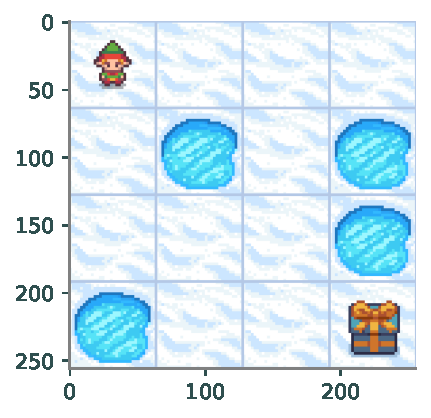
\includegraphics[width=.45\textwidth]{figures/4x4_image.pdf} &
        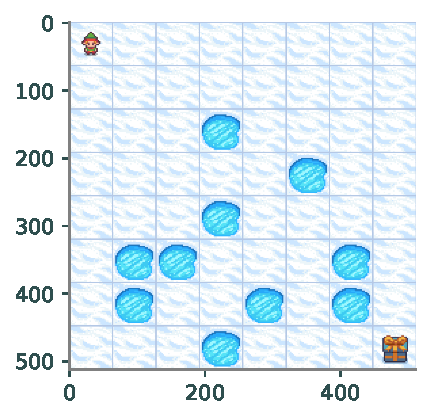
\includegraphics[width=.45\textwidth]{figures/8x8_image.pdf}
    \end{tabular}
    \caption{Default starting positions of the $4\times4$ and $8\times8$ versions of \li{"FrozenLake-v1"}}
    \label{fig:frozen_lake}
\end{figure}

\subsection*{Using Gymnasium}
The \li{'FrozenLake-v1'} environment has 3 important attributes: \li{P}, \li{observation_space.n}, and \\ \li{action_space.n}.
We can calculate the optimal policy of \li{'FrozenLake-v1'} with value iteration or policy iteration using these 3 attributes.
Since the ice is slippery, this policy will not always result in a reward of 1.

\begin{lstlisting}
>>> import gymnasium as gym

>>> # Initialize environment for 4x4 scenario
>>> env = gym.make('FrozenLake-v1', desc=None, map_name='4x4', is_slippery=True)
>>> # Find number of states and actions
>>> env.observation_space.n
16
>>> env.action_space.n
4
>>> # Get the dictionary with all the states and actions
>>> dictionary_P = env.P

>>> env.close()  # Always close the environment!
\end{lstlisting}

The attribute \li{P} is similar to the dictionary we used in the previous problems.
As already mentioned, $p(s^\prime|s,a)\leq1$, which means the set $N_{s,a}$ has more than one value.
\textbf{NOTE} if you did not implement the functions in this lab to account for this, they will not work as intended on this dictionary, which we will use for the remainder of this lab.

\begin{problem}
\label{prob:policyiter-value5}
Note first that this problem and the next are linked so you may want to read through both before starting.

Write a function called \li{frozen_lake()} that accepts a boolean \li{basic_case} defaulting to \li{True}, an integer $M$ defaulting to 1000 that indicates how many episodes of \\ \li{"FrozenLake-v1"} to run, and a boolean \li{render} defaulting to \li{False}.
If \li{basic_case} is \li{True}, run the $4\times4$ scenario.
If not, run the $8\times8$ scenario.
If \li{render} is \li{True}, render the environment by applying the argument \li{render_mode='human'} when initializing the environment.
Close the environment at the end of the function.

For each model-based algorithm, your created \li{frozen_lake()} function will also return the optimal value function array $V_*$, the optimal deterministic policy array $\pi_*$, and the average discounted reward sum for $M$ episodes.
Thus, your output is a tuple of 6 elements.
Note the two model-based algorithms are value iteration and policy iteration.
(Hint: Rendering this environment can take a long time, so only render it with small values of $M$.)

Remember that policy iteration already returns both $V_*$ and $\pi_*$ whereas value iteration only returns $V_*$.
Once you have both optimal policies, use problem\ \ref{prob:policyiter-value6} to help you obtain the average.
\end{problem}

Gymnasium environments have built-in functions that allow us to simulate each step of the scenario.
Before running a simulation in Gymnasium, always revert it to the starting position by calling the \li{reset()} function.
The function \li{step()} moves the simulation to the next state.

\begin{lstlisting}
>>> import gymnasium as gym
>>> # Initialize environment for 4x4 scenario
>>> env = gym.make('FrozenLake-v1', desc=None, map_name='4x4', is_slippery=True)

>>> # Put environment in starting state
>>> observation, info = env.reset()
>>> # Take a step in the optimal direction and update variables
>>> observation, reward, done, trunc, info = env.step(int(policy[observation]))

>>> env.close()  # Always close the environment!
\end{lstlisting}

The function \li{step()} takes integers representing different actions and returns: \li{observation}, \li{reward}, \li{done}, \li{truncated}, and \li{info}.
When we take an action, we get a new \li{observation}, or state, as well as the \li{reward} for taking that action.
If the elf falls into a hole or reaches the present, the simulation terminates (\li{done=True}).
The \li{truncated} and \li{info} values will not be used in this lab.
For more information about this environment, visit \url{gymnasium.farama.org/environments/toy_text/frozen_lake/}.

\begin{problem}
\label{prob:policyiter-value6}
Write a function \li{run_simulation()} that takes in an environment \li{env}, a deterministic policy array \li{policy}, and a discount factor $\beta$.
Calculate the total discounted reward sum of the policy for one episode of the environment (i.e.\ step through the environment until \li{done=True}).
This function will be called by \li{frozen_lake()} in\ \ref{prob:policyiter-value5}, which both initializes and closes the environment, so do not call \li{close()} in this function.
However, you should call\\ \li{reset()} at the beginning of this function, to revert the environment back to its starting position.
(Hint: When calculating the dicounted reward, use $\beta^k$ as shown in Equation\ \ref{eq:policyiter-dynopt1}.)

Next, modify \li{frozen_lake()} to call \li{run_simulation()} for both the value iteration and policy iteration for $M$ episodes.
Then, modify \li{frozen_lake()} to return the actual values of the mean total discounted reward for both policies.
(Hint: Even though you run the simulation $M$ times, you should only calculate the policies once, because each policy depends on the dictionary $P$, which does not change.)
\end{problem}

\section*{Wrapping Up Reinforcement Learning}
There a few more things to discuss before we finish this lab and move on to the last problem.
We do reserve some other important ideas to the Additional Materials section so that we can focus on the last problem.
We strongly encourage you to read through the Additional Materials section to get a better understanding of reinforcement learning.

\subsection*{Value Iteration vs.\ Policy Iteration}
An \emph{expected update} is the term used to describe the single update of value of a single state $s\in S$.
A \emph{sweep} is the term used to describe a complete iteration of an expected update for all states $s\in S$ (i.e.\ iterating through all states and updating each once).
Both value iteration and policy iteration use sweeps to find the optimal policy.
Value iteration first performs various sweeps using iterative policy evaluation.
It stops once we are within a certain tolerance of the true value function.
We then perform a single sweep using policy improvement to find the optimal policy.

On the other hand, policy iteration first performs various sweeps using policy evaluation to obtain an estimated optimal value function $V_*$.
We then perform a single sweep using policy improvement to find the optimal policy.
If the estimated optimal policy is within a certain tolerance of the previous policy, we stop.
Else, we repeat the process by performing more sweeps to first improve the estimate of the optimal value function and then to improve the policy.
This whole process of finding the optimal policy through independent alternations of policy evaluation and policy improvement (for value iteration or policy iteration) is called \emph{generalized policy iteration}.

Given these differences, policy iteration is generally more computationally expensive than value iteration.
However, policy iteration tends to yield a better policy than what value iteration yields.
Value iteration converges faster than policy iteration and is easier to implement.
Nonetheless, both algorithms are great at solving MDPs and are used in practice.

Do keep in mind that using generalized policy iteration, employing dynamic programming as we have done, while guaranteed to converge to the optimal policy, is not always the best method for solving MDPs.
We are required to sweep several times through the state space to find the optimal policy.

\subsection*{Model-Based vs.\ Model-Free}
In this lab, we have used a model-based approach to solve the \li{'FrozenLake-v1'} environment.
This means that we have used the dynamics function $p$ to find the optimal policy as well as were able to use a reward function.
This is a great way to solve MDPs when we have access to the dynamics function and reward function and know that the agent gets a full observation of the state.
However, in many cases, we do not have access to these functions.
This is where model-free methods come in.
Model-free methods still try to solve the underlying MDP, but they do not use the dynamics function or reward function to do so since they use experience to learn the optimal policy.
However, we still rely on the fact that the agent gets a full observation of the current state.
When the observation is not full, we have to use a different method called \emph{partially observable MDPs} (POMDPs).

Moreover, both methods use what is called \emph{bootstrapping}, which is the process of using estimates of value functions to improve the estimates of the same value functions we want.
These two also look ahead to the future state, compute a value, and use that value to improve the current value we are seeing.
The two method types are best for small finite MDPs.
One thing to note is that both also are computationally expensive so that they may not be the best methods for solving large MDPs.
The methods shown in these two RL labs are collectively called \emph{tabular methods} since we used tables or arrays to store the value functions and policies.

Lastly, for these two labs, we have worked with a \emph{stationary} MDP, which means that the dynamics function and reward function do not change over time.
Even when the environment is stochastic, the probabilities do not change or at least change slow enough so that the agent can learn the optimal policy.
We also assumed that we worked with a \emph{stationary} policy, which means that the policy does not change over time.
RL can get quite complicated when we have to deal with non-stationary MDPs and policies and even more so when we have to deal with POMDPs.

\begin{problem}
\label{prob:policyiter-value7}
    You will be comparing the model-free Q-learning algorithm and the model-based Value Iteration algorithm.

    Write a function called \li{model_comparison()} that accepts a parameter \li{episodes} defaulting to 1000.
    Run both algorithms on the \li{'FrozenLake-v1'} environment using the $8\times8$ grid and \li{is_slippery=True} for however many episodes \li{model_comparison()} is given.
    For each algorithm, calculate the average total discounted reward sum for however many episodes \li{model_comparison()} is given.
    Then, write a string of 2-4 sentences comparing the two algorithms using your knowledge of RL or the lab material that explains the differences in the results.
    Return a tuple of 3 elements consisting of the average total discounted reward for both algorithms and the final element being the string that you wrote.
    For consistency, keep both \li{beta} parameters at \li{1.0} to calculate the total discounted reward.
    On Q-learning, employ a linear decaying epsilon.

    To help, we have created a py file called \li{model_free_rl.py} that contains the functions \li{run_q_learn}, \li{run_simulation_table()}, and \li{epsilon_decay()}.
    The first function runs Q-learning on the \li{'FrozenLake-v1'} environment and saves a Q-table as npy file that will be used in the \li{run_simulation_table()} function to solve the \li{'FrozenLake-v1'} environment.
    There is no need to store anything from this function, so you can just run it.
    We give a breakdown of the parameters at the end.
    After you execute \li{run_q_learn}, you can comment out the line of code that executes the Q-learning algorithm since you no longer need to train it.
    Ensure the npy file was created before commenting it out.
    The npy file is named \li{q_table.npy}.

    The \li{run_simulation_table()} function is much like the problem 6 function.
    It accepts the arguments \li{env} (Gym environment) and \li{beta} a float representing the discount factor that is defaulted to 1.0.
    This function will return the total discounted reward for having followed the policy given by Q-learning for one episode of the environment.
    The code of the function already loads the npy file to extract the table, so execute this function only after you have run the Q-learning algorithm and have the npy file.

    Remember that \li{value_iteration()} only returns the value function.
    As such, you need to use another one of your functions to be able to extract the optimal policy from the value function array.
    Lastly, you will need to run the function \li{run_simulation()}, from problem\ \ref{prob:policyiter-value6}, to be able to calculate the total discounted reward of the policy produced by the value iteration algorithm.
    You may  find \li{ndarray.mean()} and list comprehension useful to compute the two 2 floats.

    You may experiment with various model hyperparameters, but when submitting the lab, ensure that all inputs use their defaults values (except for epsilon as you will linearly decay it).
    The function \li{run_q_learn} has the following 7 inputs (in order):
    \begin{itemize}
        \item \li{env} (\li{str}): The Gym environment.
        \item \li{alpha} (\li{float}): The learning rate. Defaulted to \li{0.1}.
        \item \li{gamma} (\li{float}): The discount factor. Defaulted to \li{0.6}.
        \item \li{epsilon} (\li{float}): The epsilon value for the epsilon-greedy policy. Defaulted to \li{0.1}.
        \item \li{N} (\li{int}): The number of episodes to train for. Defaulted to \li{70_000}.
        \item \li{decay} (\li{bool}): whether or not to decay the epsilon value. Defaulted to \li{False}.
        \item \li{decay_type} (\li{str}): the type of model given to \li{epsilon_decay()} in order to calculate a decaying epsilon value (\li{'linear'} or \li{'exp'} for exponential). Defaulted to \li{'linear'}.
    \end{itemize}

\end{problem}

\section*{Additional Materials}
We give a brief overview of some of the topics we did not cover in any of the labs that are important to reinforcement learning.

\subsection*{Stochastic Dynamic Programming}
\emph{Dynamic programming}, DP for short, is a method used to solve complex problems by breaking them down into simpler subproblems over time.
DP requires that a solution to the problem is able to be constructed from solutions to its subproblems\footnote{This property is called the \emph{optimal substructure} property.} and that the solved subproblems are reused several times\footnote{This property is called the \emph{overlapping subproblems} property.}.
\emph{Dynamic optimization}, or also called dynamic programming, is the process of simplyfying a decision-making problem by using these two principles of DP.
In \emph{stochastic dynamic optimization}, or stochastic dynamic programming, we use the principles of DP to solve a decision-making problem where the outcomes are partly random and partly under the control of a decision maker.
The goal in stochastic dynamic programming is to get a strategy on how to act in the face of uncertainty.
This is where the MDP comes in.
Using any of the Bellman equations, we can see that the value functions have both properties\footnote{Mainly, the calculation of the next state becomes the subproblem, and the fact that we can store that value for later use when it becomes the next state for another state is what meets the criteria.}, so we can use DP to solve the MDP.
This is why value iteration and policy iteration are considered DP methods.

\subsection*{Convergence of Value Iteration}
We proof the convergence of the value iteration we used in this lab.
A more general value iteration that uses more stochastic components can also be proved in a similar fashion.

A function $f$ that is a contraction mapping has a \emph{fixed point} $p$ such that $f(p) = p$.
Blackwell's contraction theorem can be used to show that Bellman's equation is a ``fixed point'' (it actually acts more like a fixed function in this case)
for an operator $T: L^{\infty}(X;\mathbb{R}) \to L^{\infty}(X;\mathbb{R})$ where $L^{\infty}(X;\mathbb{R})$ is the set of all bounded functions:
\begin{equation}
\label{eq:policyiter-blackwell}
T[f](s) = \max_{a \in A_s} \left\{\sum_{\bar{s}\in N_{s,a}} p(\bar{s}) \cdot \left( r(\bar{s}) + \beta f(\bar{s})\right)\right\}
\end{equation}
It can be shown that Equation\ \ref{eq:policyiter-dynopt1} is the fixed ``point'' of our operator $T$.
A result of contraction mappings is that there exists a unique solution to Equation\ \ref{eq:policyiter-blackwell}, namely

\begin{equation}
\label{eq:policyiter-val-iteration}
V_{*}^{k+1}(s_i) = T[V_*^k](s_i) = \max_{a \in A_s} \left\{\sum_{\bar{s}\in N_{s,a}}p(\bar{s}) \cdot\left( r(\bar{s}) + \beta V_*^k(\bar{s})\right)\right\}
\end{equation}
where an initial guess for $V_*^0(s)$ is used.
As $k \to \infty$, it is guaranteed that $(V_*^k(s)) \to v_*(s)$.
Because of the contraction mapping, if $V_*^{k+1}(s) = V_*^k(s) \, \, \forall \, s$, we have found the true optimal value function, $v_*(s)$.
% Using this information, we define the value iteration algorithm to find $V^*$:

% \begin{algorithm}[H]
% \begin{algorithmic}[1]
% \Procedure{Value Iteration Function}{$P, S, A, \beta, \varepsilon$, maxiter}
%     \State $V_0 \gets [V_0(s_0),V_0(s_1),\ldots,V_0(s_N)] $
%      \Comment{Common choice is $V_0(s_i)=u(s_i)$}
%     \For{$i=1,2,\dots,$\ \li{maxiter}}
%         \Comment Iterate only \li{maxiter} times at most.
%         \For{$s \in S$}
%              \State $V_{k+1}(s) = \max_{a \in A_s}\{\Sigmap(a)*(u(a) + \beta*V_k(a))]\}$
%         \EndFor
%         \If{ $||V_{k+1} - V_k|| < \varepsilon$}
%             \State \texttt{break}
%              \Comment{Stop iterating if the approximation stops changing enough.}
%         \EndIf
%     \EndFor
%     \State \pseudoli{return} $V_k$
% \EndProcedure
% \end{algorithmic}
% \caption{Value Function Iteration}
% \label{alg:ValueIteration}
% \end{algorithm}

\subsection*{Stochastic vs Deterministic Policy}
A \emph{deterministic} policy is a function $\pi: S\to A$ that maps a state $s$ to a single action $a \in A_s\subset A$ with certainty.
That is, the agent will always take the same action $a$ for a given $s$ when using a deterministic policy $\pi$.
This is why we can write $\pi(s)=a$ since only one action will be produced time and time again for a given state.
The main advantage of a deterministic policy is the easiness in implementation and interpretation.
This type of policy is best suited for environments where the agent should take the same action for a given state every single time it comes to that state or for tasks requiring precise control.

On the other hand, a \emph{stochastic} policy is a function $\pi: S\times A\to [0,1]$ where $\pi(A|S=s)$ is a possibly distinct probability distribution over the action space for a fixed state $s$.
Thus, each state can have its own probabilistic rule for selecting actions from its own action set.
Hence, $\pi(A=a|S=s)=\pi(a|s)$\footnote{This probability can also be written as $\pi(s,a)$.} is a value in the interval $[0,1]$ denoting the probability of taking action $a$ in state $s$.
The advantage of a stochastic policy is that it can capture the uncertainty of the environment but with the downside of having to learn a probability distribution for each state.
Nevertheless, this allows us to learn tasks where randomness or exploration are more common.

Do note that although we denote an action $a$ or the action space $A$ as an input for a stochastic policy, it is an output of the policy.
We use it in the input to emphasize the fact the action is uncertain as the stochastic policy can choose a completely different action.
Lastly, we can think of a deterministic policy as a stochastic policy where $\pi(a|s)=1$.

\begin{warn}
    Note that the transition probability is not the same as the probability given by some policy.
    The former is a property of the environment that cannot be changed while the latter is a property of the agent that can be changed.
\end{warn}

\subsection*{Stochastic Processes in RL}
In this lab, we worked with a stochastic environment where the outcomes of the agent's actions are not fully in the agent's control.
In the \li{'FrozenLake-v1'} environment, the agent's chosen direction is not always the direction the agent moves.
We did not consider the agent's actions to be stochastic nor did we consider the rewards to be stochastic.
The general process that can be used for more complex environments and tasks employs a stochastic policy and a stochastic reward function.

There can be a few different types of stochastic processes in RL:
\begin{itemize}
    \item The environment: This gives us either a deterministic or stochastic transition probability.
    This means that the next state is always the same for a given state-action pair or that there is a probability distribution over the next states for a given state-action pair, respectively.
    Thus, $p(s^\prime|s,a)=1,\forall (s,a)$, for deterministic, and $p(s^\prime|s,a)\leq1,\forall (s,a)$, for stochastic.

    \item The policy $\pi$: This means that the agent can either have a fixed action for a given state which implies $\pi(a|s)=P(A_t=a|S_t=s)=\pi(s)=1,\forall (s,a)$.
    Or, there is a probability distribution over actions for a given state so that $\pi(a|s)=P(A_t=a|S_t=s)\leq1, \forall s\in S$.

    \item The reward function:
    In the deterministic case, the reward function returns the same reward for the same input and is either dependent on just the current state-action pair $(s,a)$ or is dependent on the next state and current state-action pair which is the triple $(s^\prime,s,a)$.
    For stochastic, the reward function returns a probability distribution over rewards for a given $(s,a)$ or $(s^\prime,s,a)$.
\end{itemize}

The dynamics function $p$ is meant to capture the true stochastic nature of the world or environments we live in.
That is, it works with a stochastic MDP, policy, and reward.
When dealing with a deterministic reward function, we typically use the transition probability rather than the dynamics function.

With a true stochastic environment, we get the following Bellman equation for $v_\pi(s)$ as
\begin{subequations}
    \label{eq:state_value}
    \begin{align}
        v_{\pi}(s)=v(s) &= \mathbb{E} \Biggl[ \sum_{k=0}^T \beta^k r_k \Biggl\lvert S_0=s  \Biggr] \label{eq:state_value_def}\\
                        &= \sum_{a \in A_s}\pi(a|s) \sum_{s^\prime\in S^+}\sum_{r \in\mathcal{R}}p(s^\prime,r|s,a) \Bigl[r + \beta v_\pi(s^\prime) \Bigr]. \label{eq:state_value_bell}
    \end{align}
\end{subequations}

Similary, the state-action quality function $q_\pi(s,a)$ can be defined as
\begin{subequations}
    \label{eq:state_action_value}
    \begin{align}
        q_{\pi}(s,a)=q(s,a) &= \mathbb{E} \Biggl[ \sum_{k=0}^T \beta^k r_t \Biggl\lvert S_0=s, A_0=a  \Biggr] \label{eq:state_action_val_def} \\
                            &= \sum_{s^\prime\in S^+}\sum_{r \in\mathcal{R}}p(s^\prime,r|s,a) \Biggl[r + \beta \sum_{a^\prime\in A_{s^\prime}} \pi(a^\prime|s^\prime) q_\pi(s^\prime,a^\prime)\Biggr] \label{eq:state_action_val_bell}.
    \end{align}
\end{subequations}
With these two, we can form the relationship
\begin{align}
    v_\pi(s) = \sum_{a\in A_s} \pi(a|s)q_{\pi}(s,a).
    \label{eq:value_quality_relationship}
\end{align}

We can then get the Bellman optimality for $v_*$
\begin{align}
    v_*(s) &= \max_{a\in A_s} q_{\pi_*}(s,a) \nonumber \\
           &= \max_{a\in A_s} \sum_{s^\prime\in S^+}\sum_{r\in\mathcal{R}}p(s^\prime,r|s,a) \Bigl[r + \beta v_*(s^\prime)\Bigr],
    \label{eq:state_value_bell_optimal}
\end{align}
and the action-value as
\begin{align}
    q_*(s,a) &= \mathbb{E}[r_0 + \beta\max_{a^\prime\in A_s} q_*(s_1,a^\prime)|S_0=s,A_0=a] \nonumber \\\
             &= \sum_{s^\prime\in S^+} \sum_{r\in\mathcal{R}} p(s^\prime,r|s,a) \Bigl[r + \beta\max_{a^\prime\in A_{s^\prime}} q_*(s^\prime,a^\prime)\Bigr].
    \label{eq:action_value_bell_optimal}
\end{align}
The remainder of the other functions for a stochastic process that are similar to those used in the lab can be derived from these equations.

\subsection*{Deterministic Reward Function}
In the lab, we assumed that the reward function was deterministic.
Specifically, we worked with a function that had a reward dependent not only on the current state-action pair $(s,a)$ but also on the next state $s^\prime$.
This was the reward function of three inputs $r(s^\prime,s,a)$.

In other cases, the reward function can be dependent only on the current state-action pair $(s,a)$.
Using the dynamics function $p$, we can also compute the reward function of two inputs $r:S\times A\to\mathbb{R}$ as
\begin{align}
    r(s,a)=r_t(s,a) = \mathbb{E}[R_{t}|S_t=s, A_t=a] = \sum_{r\in\mathcal{R}} r \sum_{s^\prime\in S} p(s^\prime, r|s,a).
    \label{eq:MDP_reward_two_inputs}
\end{align}
This tells us the expected reward for taking action $a$ in state $s$ at timestep $t$.

Do note that $r(s^\prime,s,a)$ and $r(s,a)$ are not necessarily the same as they have different uses.
When we care about going to a specific state after taking a specific action, we use $r(s^\prime,s,a)$.
When we care about the reward for taking a specific action in a specific state, we use $r(s,a)$.

\subsection*{Solving the Optimization Problem}
For each state, there may be multiple actions that maximize the value function in the Bellman optimality equation (recall the definition of argmax).
Thus, any policy that assigns a nonzero probability to these actions is an optimal policy.
That is, any policy that is \emph{greedy}\footnote{By greedy we mean any search or decision procedure that selects alternatives based on local or immediate considerations without considering the possibility that such a selection may prevent future access to even better alternatives.} with respect to the optimal value function is an optimal policy.
A greedy policy only selects the action that maximizes the value function only in the short term, specifically only optimizing the expected future rewards of the next timestep, but the nature of $v_*$ already considers the long-term rewards of all possible future behavior making it available to each state immediately.
Hence, given the Bellman optimality equation for $v_*(s)$ (\ref{eq:state_value_bell_optimal}), we can simply use
\begin{align}
    \pi_*=\pi_*(s)=\underset{a\in A_s}{\argmax}\text{ } v_*(s).
    \label{eq:optimal_policy_value_def}
\end{align}

When we have the optimal action-value function, we can use
\begin{align}
    \pi_*=\pi_*(s)=\underset{a\in A_s}{\argmax}\text{ } q_*(s,a).
    \label{eq:optimal_policy_quality_def}
\end{align}
In this case, there is no need to perform some greedy search since the optimal action-value function selects optimal actions without having to know anything about possible successor states and their respective values.
In general, the optimal policy is usually deterministic since we only care about choosing one of the many optimal actions available (or the only optimal action available).
Should we have started with a stochastic policy and want it to remain stochastic, we need only assign each optimal action any probability we want as long as the suboptimal actions are given a probability of 0.
This will keep the policy stochastic but still optimal.
But, we can always just choose one of the optimal actions and assign it a probability of 1 to make the stochastic policy deterministic.

\subsection*{Closer Look Into Policy Improvement}
In the section on policy improvement, we mentioned that policy improvement finds the optimal policy.
We had supposed that there was a new policy $\pi^\prime$ that was better than the old policy $\pi$.
But what if there was a new policy that is just as good as the old policy but not better than the current policy $\pi$?
Then, $v_\pi = v_{\pi^\prime}$, so that from
\begin{align*}
    \pi^\prime(a|s)=\underset{a\in A_s}{\argmax}\text{ } q_\pi(s,a)= \underset{a\in A_s}{\argmax} \sum_{s^\prime\in S^+} \sum_{r\in\mathcal{R}} p(s^\prime,r|s,a)[r+\beta v_{\pi}(s^\prime)] \nonumber
\end{align*}, we have
\begin{align*}
    v_{\pi^\prime} = \underset{a\in A_s}{\max}\text{ } \sum_{s^\prime\in S^+} \sum_{r\in\mathcal{R}} p(s^\prime,r|s,a) [r+\gamma v_{\pi^\prime}(s^\prime)]. \nonumber
\end{align*}
This is the Bellman optimality equation so that $\pi^\prime$ is an optimal policy as is $\pi$.
Thus policy improvement does find the optimal policy except in the case where the original policy is optimal so that we do not have to improve the current policy.

\subsection*{When Should I Use RL?}
Tom Mitchel defined machine learning as
\begin{quote}
    A computer program is said to learn from experience $E$ with respect to some class of tasks $T$ and performance measure $P$, if its performance at tasks in $T$, as measured by $P$, improves with experience $E$.
\end{quote}
There are, in general, three types of learning: supervised learning, unsupervised learning, and reinforcement learning.

In \emph{supervised learning}, the computer is given a set of inputs and outputs that have been already been given some context of a relationship and is asked to learn the mapping between the two.
Whereas in \emph{unsupervised learning}, the computer is given a set of inputs and outputs and is asked to find the structure or patterns in the data without having any context of any sort of relationship in the data.
While these two types of learning are great for many tasks, they do not work well when the computer has to interact with the environment to learn a task.
In RL, we are concerned about finding any structure or patterns nor are we concerned about finding a mapping between inputs and outputs.
We are strictly concerned with how the computer ought to take actions in an environment to maximize some notion of a cumulative reward.

Typically RL is better used when the algorithm needs to make sequential decisions in an environment.
This is because RL is great at learning how to make decisions in an environment where the agent can interact with the environment.
Typically RL is best in these types of environments where we have an existing decision-making model that we want to improve or when we have a decision-making model that we want to learn from scratch through interaction.
RL is also great when the agent can receive feedback from the environment in the form of a reward.
Thus, we need to be able to define a reward function that tells the agent how well it is doing and not run into the \emph{reward engineering problem}.

Morever, RL is great when the agent can learn from its mistakes and improve its decision-making process.
Thus, when we can afford to have the agent make mistakes and learn from them, online RL is a great tool to use.
But when we cannot afford to have the agent make mistakes, offline RL is a better tool to use so we must be able to have a dataset of the environment that the agent can learn from.

\subsection*{Challenges in RL}
We talked about the exploration-exploitation trade-off in the last lab.
RL faces other problems that must be dealt with whenever you are formulating a problem as an RL problem.
Here are some of the challenges in RL:
\begin{itemize}
    \item \emph{Credit Assignment Problem}: This is the challenge of determining which actions an agent took that led to a particular reward.
    This is a problem because the agent may have taken many actions before receiving a reward.
    The agent must determine which of these actions led to the reward.
    It could be that the reward was due to a combination of actions or that the reward was due to an action that was taken a long time ago.
    Moreover, this also does not mean that other actions were not important as those actions could have set up the agent to receive the reward while not directly giving the reward.

    \item \emph{Reward Engineering Problem}: This is the process of designing a good reward function that encourages the desired behavior in the agent.
    The reward should reflect the desired goal we want the agent to achieve.
    The reward is not a place to give the agent new information about the environment.
    It should only be used to tell the agent how well it is doing.

    \item \emph{Generalization Problem}: This is the ability of an agent to apply what it has learned to new and previously unseen situations.
    This is a problem because the agent may have learned a policy that works well in the training environment but does not work well in the testing environment.
    It also arises when the agent has to learn a policy in an arbitrarily large state space.
    The agent must be able to generalize its policy to all states in the state space but may not have visited all states during training.

    \item \emph{Sample Efficiency Problem}: This refers to the ability of an RL agent to learn an optimal policy with a limited number of interactions with the environment.
    Many RL algorithms require a large number of interactions with the environment (or a large dataset of the environment) to learn an optimal policy.
    This is a problem because in many real-world applications, the agent cannot interact with the environment an unlimited number of times.
\end{itemize}

\subsection*{Futher Reading and Resources}
Reinforcement learning is a vast field with many different algorithms and techniques and applications.
The following are some resources that can help you learn more about reinforcement learning.
Note that some of these are available online for free through various universities or by the publishers or authors themselves.
\begin{itemize}
    \item \emph{Reinforcement Learning: An Introduction}, 2nd edition, 2018, by Richard S. Sutton and Andrew G. Barto is a classic book covering the basics of reinforcement learning and algorithms.
    It also gives a good overview of the field and the math behind it.
    The only prerequisite knowledge is the material you have learned in Volume 2 textbook.
    \item \emph{Algorithms for Reinforcement Learning}, 2009, by Csaba Szepesvári is a book that covers many different algorithms in reinforcement learning strictly and rigorously from a mathematical perspective.
    It does not contain many implementations or applications, but it does cover the strengths and weaknesses of many algorithms as well as the math behind them and what is known or unknown about them.
    The material therein is more advanced than the Sutton and Barto book, so knowledge of Volume 1 and 2 textbooks is recommended.
    \item \emph{Data-Driven Science and Engineering: Machine Learning, Dynamical Systems, and Control}, 2nd edition, 2022, by Steven L. Brunton and J. Nathan Kutz is a book that brings together machine learning, mathematics, and physics to integrate modeling of dynamical systems.
    The book contains chapters on reinforcement learning and deep reinforcement learning, as well as many other topics in machine learning.
    Dr. Brunton has a \href{https://www.youtube.com/@Eigensteve}{YouTube channel} where he covers some of the material in the book, including a playlist on \href{https://www.youtube.com/watch?v=0MNVhXEX9to&list=PLMrJAkhIeNNQe1JXNvaFvURxGY4gE9k74}{reinforcement learning}.
    \item \emph{Reinforcement Learning and Optimal Control}, 2019, by Dimitri P. Bertsekas is a book that covers reinforcement learning and optimal control from a mathematical perspective and using dynamic programming.


\end{itemize}


% Old lab content -------------------------------------------------------------------
\begin{comment}
\newpage
%
%
%%\begin{equation}
%%\label{eq:policyiter-bellman1}
%%V(w_i) = \max_{c \in [0,w_i]} u(c) + \beta V(w_i-c)
%%\end{equation}
%%It is common to make the substitution $w_i' = w_i - c$ in \eqref{eq:policyiter-bellman1} to obtain the %following.
%\begin{equation}
%\label{eq:policyiter-bellman2}
%V(w_i) = \max_{w_j \in [0,w_i]} u(w_i-w_j) + \beta V(w_j).
%\end{equation}
%
%Notice that \eqref{eq:policyiter-bellman2} is similar to the value function given in the dynamic programming lab.
%%Note that \eqref{eq:policyiter-bellman1} requires finding $c$, how much cake to consume in each period.
%%The variable $c$ is commonly described as the \emph{action} to take when we have $w_i$ cake.
%
%
%\subsection*{Convergence of Value Iteration}
%
%A function $f$ that is a contraction mapping has a fixed point $p$ such that $f(p) = p$.
%Blackwell's contraction theorem can be used to show that Bellman's equation is a ``fixed point'' (it actually acts more like a fixed function in this case)
%for an operator $T: L^{\infty}(X;\mathbb{R}) \to L^{\infty}(X;\mathbb{R})$ where $L^{\infty}(X;\mathbb{R})$ is the set of all bounded functions:
%\begin{equation}
%\label{eq:policyiter-blackwell}
%[T(f)](w) = \max_{w_j \in [0,w]} u(w-w_j) + \beta f(w_j).
%\end{equation}
%It can be shown that (\ref{eq:policyiter-bellman2}) is the "fixed point" of our operator $T$.
%A result of contraction mappings is that there exists a unique solution to (\ref{eq:policyiter-blackwell}).
%
%A powerful property of contraction mappings is that the fixed point can be found by applying the function repeatedly to some initial point in our domain.
%That is, if $f:X \to X$ is our contraction mapping, with fixed point $p \in X$, we can find $p$ by randomly choosing $x \in X$ and repeatedly applying the function $f$ to our point.
%This can be expressed as
%\begin{align*}
%f^{M}(x) = f \circ f \cdots \circ f(x) = p
%\end{align*}
%for some M.  Here M is dependent on both the initial guess $x$ and the discount factor of the contraction mapping, which correspond to $V_0$ and $\beta$ in dynamic optimization.
%
%In the case of dynamic optimization, this implies that we can converge to the true value function $V^*(w)$ by using the following equation:
%\begin{equation}
%\label{eq:policyiter-val_iteration}
%V_{k+1}(w_i) = [T(V_k)](w_i) = \max_{w_j \in [0,w_i]} u(w_i-w_j) + \beta V_k(w_j) \, \, \forall \, w_i,
%\end{equation}
%
%where an initial guess for $V_0(w)$ is used.
%As $k \to \infty$, it is guaranteed that $(V_k(w)) \to V^*(w)$.
%Because of the contraction mapping, if $V_{k+1}(w) = V_k(w) \, \, \forall \, w$, we have found the true value function, $V^*(w)$.
%Using this information, we define the value iteration algorithm to find $V^*$:
%
%
%
%
%\begin{algorithm}[H]
%\begin{algorithmic}[1]
%\Procedure{Value Iteration Function}{$\beta, N, W, u(x), \varepsilon$, maxiter}
%    \State $w \gets [0, \frac{W}{N},\ldots, W]$
%      \Comment{Divide $W$ into $N$ equally sized pieces}
%    \State $V_0 \gets [V_0(w_0),V_0(w_1),\ldots,V_0(w_N)] $
%     \Comment{Common choice is $V_0(w_i)=u(w_i)$}
%    \For{$i=1,2,\dots,$\ \li{maxiter}}
%        \Comment Iterate only \li{maxiter} times at most.
%        \For{$w_i \in w$}
%            \State $V_{k+1}(w_i) = \max_{w_j \in \mathbf{w} \, | \, w_j \leq w_i} u(w_i-w_j) + \beta V_k(w_j)$
%        \EndFor
%        \If{ $||V_{k+1} - V_k|| < \varepsilon$}
%            \State \texttt{break}
%             \Comment{Stop iterating if the approximation stops changing enough.}
%        \EndIf
%    \EndFor
%    \State \pseudoli{return} $V_k$
%\EndProcedure
%\end{algorithmic}
%\caption{Value Function Iteration}
%\label{alg:ValueIteration}
%\end{algorithm}
%
%Most iterative algorithms have a \li{max\_iter} parameter that will terminate the algorithm after \li{max\_iter} iterations regardless of whether or not it has converged.
%This is because even though we have guaranteed convergence, we might have a convergence rate that is too slow to be useful.
%However, generally this algorithm will converge much faster than computing the true value function using dynamic programming as in Finite Value Iteration.
%
%\begin{warn} % Notation warning
%Note that $w_j \leq w_i$, because we can never have more cake at a later period; cake can only be consumed, not created.
%\end{warn}
%
%\begin{problem}
%\label{prob:policyiter-value1}
%Write a function called \li{value_iteration()} that will accept a numpy array representing the initial vector $V_0$, a discount factor $\beta \in (0,1)$,
%the number of states to split $\mathbf{w}$ into $N$, the amount of initial cake $W$, a utility function $u(x)$,
%the tolerance amount $\epsilon$, and the maximum number of iterations \li{max\_iter}.
%Perform value iteration until $\|V_{k+1} - V_{k}\| < \epsilon$ or $k > $ \li{max\_iter}.
%Return the final vector representing $V^*$.
%
%It is useful for our function to accept $V_0$ as a parameter instead of calculating an initial guess inside our function, so that we can try different initial states for $V_0$.
%
%Test your function with the parameters $N=400$, $\beta=.995$, $u(x)=\sqrt{x}$, $W=1$.
%Try different values for $V_0$ and see if you get the same value for $V^*(W)$ (The value should be approximately 9.4988).
%% Question to consider:
%How do different initial guesses for $V_0$ affect the number of iterations required for convergence?
%\end{problem}
%
%
%\subsection*{Policy Vector}
%
%The value function $V^*(w_i)$ that we found describes how much utility $w_i$ will yield over time, thus $V^*(W)$ is the optimal value for our problem:
%\begin{align*}
%  V^*(W) = \max_{c_t}  & \sum_{t=0}^T \beta^t u(c_t), \\
%  \mbox{subject to } & \sum_{t=0}^T c_t = W ,\\
%  & c_t \geq 0.
%\end{align*}
%Although $V^*(W)$ is the solution, it is usually more important to know which sequence of $(c_t)_{t=0}^T$ yields the solution.
%This sequence is known as the \emph{policy vector} $\mathbf{c} = [c_0, c_1, \ldots, c_T]$ that corresponds to eating $c_i$ cake at time $t=i$.
%
%If this were a truly infinite problem, $\mathbf{c}$ would be impossible to calculate; there would be an infinite number of time periods.
%Fortunately, in the cake-eating problem, we will never have more than $N$ time periods.
%This happens because it is never optimal to eat $0$ pieces of cake in a single time period.
%The discount factor $\beta$ means at least $1$ piece must be eaten at each step.
%It is important to note that the length of $\mathbf{c}$ changes depending on what $\beta$ is.
%When $\beta = 0$, for example, only the first time period matters because all the rest will yield zero utility.
%So when $\beta = 0$, $T = 0$ and the length of $\mathbf{c}$ is $1$.
%As the value of $\beta$ gets closer to $1$, $T$ increases as well.
%
%The policy vector, $\mathbf{c}$, is found by using the policy function: $\pi : \mathbb{R} \to \mathbb{R}$ which has the constraint $0 \leq \pi(w_i) \leq w_i \, \, \forall \, i.$
%$\pi(w_i)$ is the amount of cake to save for the next period, given we started with $w_i$ cake.
%In \eqref{eq:policyiter-val_iteration}, this was represented by $w_j$.
%
%Because $\pi(w_i)$ is the amount of cake saved until next period, we can use $V^*(W)$ and modify the Bellman equation to find $\pi$:
%\begin{equation}
%\label{eq:policyiter-pol_func}
%\pi(w_i) = \argmax_{w_j \in \mathbf{w} \, | \, w_j\leq w_i} u(w_i-w_j) + \beta V^*(w_j) \, \, \forall \, i.
%\end{equation}
%For our purposes, the policy function will be represented as a vector $\mathbf{\pi}$.
%This is convenient because in practice it is infeasible to code a functional representation for $\pi$.
%$\mathbf{\pi}_i$ dictates how many pieces of cake to save for the next period if we currently have $i$ pieces of cake.
%
%Once we have a vectorized representation of the policy function, $\pi$, we can use it to calculate the policy vector $\mathbf{c}$ using the relationship:
%\begin{align*}
%  c_t = w^{(t)} - \pi(w^{(t)})), \\
%  \mbox{where } w^{(t+1)} = \pi(w^{(t)}), \\
%  \mbox{and } w^{(0)} = W.
%\end{align*}
%
%For example, assume $w = [0,.1,.2,\ldots,1]$ and $\pi = [0, 0, 1, 2, 2, 3, 3, 4, 4, 5, 5]$.
%This means that if we have $7$ pieces of cake remaining, $\pi(7) = 4$ so we should save $4$ pieces of cake for the next time period.
%At $t=0$, $w^0=1=w_{10}$, so there are $10$ pieces of cake.
%$\pi(10) = 5$, so at time $0$, we want to save $5$ pieces of the cake.
%Then $c_0=10-5=5$, and we consume half of the cake.
%To calculate $c_1$, observe that $w^1= \pi(10)=5$.
%$\pi(w^1) = \pi(5) = 3$.
%So at time $2$, we eat $5-3=2$ pieces of cake, or $w_3=.2$ of the total cake.
%The resulting policy vector is $\mathbf{c} = [0.5,0.2,0.1,0.1,0.1]$.
%
%\begin{warn}
%$w^{(t)}$ represents a time index, how much cake we have at time $t$, not to be confused with $w_i$, the numeric value of having $i$ pieces.
%\end{warn}
%
%\begin{problem}
%Write a helper function called \li{extract_policy_vector()} that will accept an array of discretized values $\mathbf{w}$, and a vector representing a policy function $\pi$.
%Return the policy vector $\mathbf{c}$ that determines how much cake should be eaten at each time step.
%
%Test your function with $\mathbf{w} = [0,.1,.2,\ldots,1]$ and $\pi = [0, 0, 1, 2, 2, 3, 3, 4, 4, 5, 5]$, as in the example above.
%\end{problem}
%
%\begin{problem}
%Modify \li{value_iteration()} to return the true value function $V_{k+1}$ and the corresponding policy vector $\mathbf{c}$.
%\\(Hint: Use \eqref{eq:policyiter-pol_func} to find the policy function and then call
%\li{extract_policy_vector()} inside of \li{value_iteration()}).
%\end{problem}
%
%\section*{Policy Function Iteration}
%For infinite horizon dynamic programming problems, it can be shown that value function iteration converges relative to the discount factor, $\beta$.
%As $\beta$ approaches $1$, the number of iterations increases dramatically.
%As mentioned earlier $\beta$ is usually close to $1$, which means this algorithm can converge slowly.
%In Problem \ref{prob:policyiter-value1} you should have noticed that runtime was significantly longer to run for larger $N$ or
%$\beta$ closer to 1.
%
%In value iteration, we used an initial guess for the value function, $V_0$ and used (\ref{eq:policyiter-bellman2}) to iterate towards the true value function.
%Once we achieved a good enough approximation for $V^*$, we recovered the true policy function $\pi$.
%Instead of iterating on our value function, we can instead make an initial guess for the policy function, $\pi_0$, and use this to iterate toward the true policy function, called policy iteration.
%We do so by taking advantage of the definition of the value function, where we assume that our policy function yields the most optimal result.
%
%That is, given a specific policy function $\pi_k(W)$, we can modify \eqref{eq:policyiter-bellman2} by assuming that the policy function is the optimal choice.
%\begin{align*}
%  V_k(w_i) = \max_{w_j\in [0,w_i]} u(w_i-w_j) + \beta V_k(w_j) = u(w_i - \pi_k(w_i)) + \beta V_k(\pi_k(w_i)). \\
%\end{align*}
%This is because $w_j$ is the amount of cake we should have left over after $t=i$, which is $\pi(w_i)$.
%Because the value function is defined recursively,
%\begin{equation}
%  \label{eq:policyiter-val_from_policy}
%V_k(W) = \sum_{t=0}^{\infty}\beta^t u(\pi_k^t(W) - \pi_k^{t+1}(W)), \\
%\end{equation}
%where $\pi_k^t(W)$ means applying $\pi_k$ t times, and $\pi_k^0(W) = W$.
%Recall that \eqref{eq:policyiter-val_from_policy} will terminate in a finite number of steps (because we will eventually run out of cake to eat).
%Fortunately, in cake-eating, \eqref{eq:policyiter-val_from_policy} can alternatively be calculated by using dynamic programming, \eqref{eq:policyiter-bellman2} which defines the relationship as:
%\begin{equation}
%  \label{eq:policyiter-fast_val_from_policy}
%  V_k(W) = u(\pi_k^t(W) - \pi_k^{t+1}(W)) + \beta V_k(\pi_k^{t+1}(W)).
%\end{equation}
%
%This happens because $\pi_k^{t+1}(W) < W$, with the initial condition that $V_k(0) = 0$.
%Thus, given an initial guess for our policy function, $\pi_0$, we calculate the corresponding value function using (\ref{eq:policyiter-val_from_policy}), and then use \eqref{eq:policyiter-pol_func} to improve our policy function.
%The algorithm for policy function iteration can be summarized as follows:
%
%
%
%\begin{algorithm}[H]
%\begin{algorithmic}[1]
%\Procedure{Policy Iteration Function}{$\beta, N, W, u(x), \varepsilon$, maxiter}
%    \State $w \gets [0, \frac{W}{N},\ldots, W]$
%      \Comment{Divide $W$ into $N$ equally sized pieces}
%    \State $\pi_0 \gets [\pi_0(w_0),\pi_0(w_1),\ldots,\pi_0(w_N)] $
%     \Comment{Common choice is $\pi_0(w_i)=w_{i-1}$ with $\pi_0(0)=0$}
%    \For{$i=1,2,\dots,$\ \li{maxiter}}
%        \Comment Iterate only \li{maxiter} times at most.
%        \For{$w_i \in \mathbf{w}$}
%            \State $V_{k}(w_i) = u(\pi_k^t(w_i) - \pi_k^{t+1}(w_i)) + \beta V_k(\pi_k^{t+1}(w_i))$
%            \State $\pi_{k+1}(w_i) = \argmax_{w_j \in \mathbf{w} \, | \, w_j \leq w_i} u(w_i-w_j) + \beta V_k(w_j)$
%        \EndFor
%        \If{ $||\pi_{k+1} - V_k|| < \varepsilon$}
%            \State \texttt{break}
%             \Comment{Stop iterating if the approximation stops changing enough.}
%        \EndIf
%    \EndFor
%    \State \pseudoli{return} $V_k, \pi$
%\EndProcedure
%\end{algorithmic}
%\caption{Policy Iteration}
%\label{alg:PolicyIteration}
%\end{algorithm}
%




% TODO: This may be a more efficient way of finding the value function $V_k$. Should we implement this?
% In order to compute the value function, $V_k$ corresponding to a given policy $\pi_k$, we must solve
% \begin{equation}
% \label{Val_Fun}
% V_k(W) = u(W-W') + \beta V_k(W')
% \end{equation}
% for $V_k$.
%
% As always, we take a discrete approximation to $W$, obtaining a length $N$ vector
% \[
% w = (w_0, w_1, w_2, \ldots, w_N)
% \]
% giving the possible cake quantities.
% The variable $W'$ becomes $w' = \pi_k(w)$.
% Once we have done this, equation \eqref{Val_Fun} is a linear system which we can rewrite as
% \begin{equation*}
% V_k(w) = u(w-w') + \beta QV_k(w)
% \end{equation*}
% where $Q$ is the $N\times N$ matrix
% \begin{equation*}
% Q_{ij} = \left\{
%      \begin{array}{ll}
%        1 & \text{if} \quad  w_i' = w_j\\
%        0 & \text{otherwise.}
%      \end{array}
%    \right.
% \end{equation*}
% Solving this system of equations, we have $V_k(w) = (I-\beta Q)^{-1}u(w-w')$.
% Although $Q$ may be large, we can take advantage of the fact that it is sparse, containing only $N$ nonzero entries out of $N^2$ total entries.

%\begin{problem}
%\label{prob:cake_eating_policyfun}
%Write a function called \li{policy_iteration()} that will accept a numpy array representing the initial vector $\pi_0$, a discount factor $\beta \in (0,1)$,
%the number of states to split $\mathbf{w}$ into $N$, the initial amount of initial cake $W_{max}$, a utility function $u(x)$, the convergence tolerance $\epsilon$, and the maximum number of iterations \li{max_iter}.
%Perform Policy Iteration until $\|\pi_{k+1} - \pi_{k}\|_\infty < \epsilon$ or $n > $ \li{max_iter}.
%Return the final vector representing $V_k$ as well as the policy vector $\mathbf{c}$.
%
%Test your policy iteration by calling \li{value_iteration()} and \li{policy_iteration()} using the same values for $\beta$, $N$, $W_{max}$, and $u(x)$.
%The value functions returned should be close to equal (use \li{np.allclose()}), and the policy vectors $\mathbf{c}$ should be identical.

% How many iterations does Policy Iteration take to converge?
% How does this compare to the number of iterations Value Iteration takes?

% TODO: Is this a more efficient way to do it?
% You will still need to pre-compute all values of $u(W-W')$, storing these in an $N \times N$ array. Make sure, as before,
% that the upper triangular entries are set to large negative values, so that we don't choose to consume more cake than is
% available. In the code snippets below, we will refer to this array as \li{U}.
%
% You may also find it convenient to not track the approximated policy function $\psi_k$ directly during the iteration, but
% rather to have a length $N$ array \li{psi_ind}, whose $i$-th entry gives the index of $w_i'$ relative to the discrete approximation
% $w$. Thus, rather than initializing a policy function $\psi_0$ directly, you can initialize it indirectly by setting, for example,
% \begin{lstlisting}
% >>> psi_ind = np.arange(N)
% \end{lstlisting}
% which corresponds to an initial policy $\psi_0(W) = W$.
% The policy function vector can be obtained from \li{psi_ind} by simply slicing \li{w} as follows:
% \begin{lstlisting}
% >>> psi = wpsi_ind]
% \end{lstlisting}
%
% In order to take advantage of the sparse matrices $I$ and $Q$, use the following imports from the SciPy \li{sparse} library.
% \begin{lstlisting}
% >>> from scipy import sparse
% >>> from scipy.sparse import linalg
% \end{lstlisting}
% and the following code to initialize $I$ (outside the loop)
% \begin{lstlisting}
% >>> I = sparse.identity(N, format='csr')
% >>> rows = np.arange(0, N)
% \end{lstlisting}
% and $Q$ (inside the loop)
% \begin{lstlisting}
% >>> columns = psi_ind
% >>> data = np.ones(N)
% >>> Q = sparse.coo_array((data, (rows,columns)), shape=(N,N))
% >>> Q = Q.tocsr()
% \end{lstlisting}
% Rather than compute $(I-\beta Q)^{-1}$ directly, use Scipy's sparse solver
% \begin{lstlisting}
% V = linalg.spsolve(I-beta*Q, u(w-wpsi_ind]))
% \end{lstlisting}
% where \li{u} is the square root function.
%
% In each iteration, we update \li{psi_indices} much as we did in the value function iteration algorithm:
% \begin{lstlisting}
% >>> psi_ind = np.argmax(U + beta*V, axis=1)
% \end{lstlisting}
% where we assume \li{V} has shape \li{(1,N)}.
%
% Use the 2-norm when computing $\|\psi_{k+1} - \psi_k\|$, and set the tolerance to $\delta = 1e-9$.
%
% Take $N = 1000$ and $\beta = .95$.
%\end{problem}

%%%%%%%%%%%%%% MPI %%%%%%%%%%%%%%%%%%%% Uncomment when we fix it.
% \section*{Modified Policy Function Iteration}
% Although policy iteration converges in fewer iterations, computing $V_k$ using (\ref{eq:policyiter-val_from_policy}) at each iteration can be quite costly, especially for problems with large $N$.
% Thus policy iteration converges slowly relative primarily to $N$, and value iteration converges slowly relative primarily to $\beta$.
% It turns out there is a hybrid method called modified policy function iteration that seeks to simultaneously minimize these disadvantages by performing policy iteration and value iteration together.
%
% Modified policy iteration is identical to policy iteration, with the addition of one extra step.
% Before \ref{alg:computing_pi_k} of the policy iteration algorithm, take the $V_k$ computed in step \ref{alg:computing_V_k} and perform value iteration with \li{max_iter}$=m$ using $V_k$ as the initial guess.
% This is faster than solving for the exact value function for large state spaces at every single iteration.
% There is no strict rule on the value of $m$, but typically $m \in [5,15]$ work well.
%
% Thus the algorithm for modified policy iteration can be summarized as follows:
% \begin{enumerate}
%   \item Discretize the space into $N$ equal sized pieces: $\mathbf{w} = \left[w_0, w_1, \ldots, w_N\right]$ where $w_0 = 0, \, \, w_N = W_{max}$.
%   \item Choose an initial vector to represent $\pi_0$: $\left[\pi_0(w_0), \pi_0(w_1), \ldots, \pi_0(w_N)\right]$
%             A common initial choice for $\pi_0$ is $\pi_0(w_i) = w_{i-1}$, meaning we save $w_{i-1}$ pieces, and $\pi_0(w_0) = 0$.
%   \item For $k = 1, 2, \ldots,$ \li{max\_iter}:
%   \begin{enumerate}
%     \item \label{alg:computing_V_k2} For each $w_i \in \mathbf{w}$ compute the value function $V_k(w_i)$ using (\ref{eq:policyiter-val_from_policy}).
%     \item \label{alg:value_iteration2} Call \li{value_iteration()} with $V_k$ as the initial guess, and use $max\_iter = m$, for some $m$.
%         Use the value function that it returns ($\hat{V_k}$) as the value function to use in \ref{alg:computing_pi_k2}.
%     \item \label{alg:computing_pi_k2} For each $w_i \in \mathbf{w}$ calculate $\pi_{k+1}(w_i) = \argmax_{W' \in \mathbf{w} \, | \, W' \leq w_i} u(w_i-W') + \beta \hat{V_k}(W')$.
%     \item If $\| \pi_{k+1} - \pi_k \| < \epsilon,$ terminate early.
%   \end{enumerate}
% \end{enumerate}
% Note that our previous methods, value iteration, and policy iteration are like two sides of our algorithm: iterating on the value function or iterating on the policy function.
% Modified policy function does a combination of both, attempting to take advantage of both methods while trying to avoid their disadvantages.
% Because modified policy iteration takes only slightly more work to code compared to value iteration and policy iteration, it is often preferred in practice.
% Modified policy iteration usually performs better than value iteration or policy iteration.
%
% \begin{problem}
% Write a function \li{modified_policy_iteration()} that takes the same arguments as \li{policy_iteration()}, along
% with an additional keyword argument $m$, which indicates the number of iterations of value iteration to do at each iteration of policy iteration.
% Return the converged value function and policy vector.
%
% Much of the code in \li{policy_iteration()} can be re-used, you just need to implement the extra step introduced by modified policy iteration.
% This is why the \li{value_iteration()} function accepts $V_0$ as a parameter, it makes implementing MPI much simpler.


% TODO: Based on other TODOS, do we want to solve the linear system?
% The key differences are as follows.
% First, you do not need to initialize the sparse arrays $I$ and $Q$ in the modified policy function iteration.
% Secondly, rather than solving a linear system of equations to obtain the value function, you will loop
% the equation
% \begin{lstlisting}
% >>> V = u(w - wpsi_ind]) + beta*Vpsi_ind]
% \end{lstlisting}
% $m$ times in each iteration. Notice how this line of code corresponds with Equation \eqref{Val_Fun}, where
% \li{w} represents $W$, \li{wpsi_ind]} represents $W'$, and \li{Vpsi_ind]} represents $V(W')$.
%
% The remainder of the code should be unchanged.
%\end{problem}
%%%%%%%%%%%%%%%%%%%% END OF MPI SECTION AND PROBLEM %%%%%%%%%%%%%%%%%%%%%%

%\begin{problem}
%Solve the cake eating problem with both value iteration and policy iteration for various values of $\beta$ and compare how long each method takes.
%% Each final $V^*$ should be \emph{np.allclose} and your policy vectors $\mathbf{c}$ should be identical for both methods.
%Use $N=1000$ as the number of grid points for $\mathbf{w}$ and $\beta = [.95, .975, .99, .995]$.
%
%It is important to use feasible initial guesses in each case in order to make the results comparable.
%A good initial guess greatly affects the number of iterations required for convergence.
%Use $V_0(w_i) = u(w_i)$ for value iteration, and $\pi_0(w_i) = w_{i-1}$, with $\pi_0(w_0) = 0$ for policy iteration.
%\\(Hint: set \li{max\_iter} high enough for each method so that the functions actually converge; large values of $\beta$ may require several hundred iterations for value iteration.)
%
%Graph the results for each method with $\beta$ on the x-axis and time on the y-axis.
%Compare your results to the following figure.
%
%\begin{figure}[H] % This figure plots the time each method takes to converge
%\centering        % use width=.7\textwidth to size the figure.
%    \includegraphics[width=.7\textwidth]{figures/comparing_methods.pdf}
%    % \caption{Comparing each method for various values of $\beta$.}
%    \label{fig:basic1}
%\end{figure}
%
%% You were not asked to compare these functions to the \li{find_policy()} function written in Finite Value Iteration because it is significantly slower than these iterative methods.
%\end{problem}

\begin{comment}
\newpage

\section*{Additional Material}
Perhaps here we can talk a bit about truly infinite MDPs such as choosing an optimal path through some kind of grid.

Or we could spend time talking about Stochastic MDPs where we introduce probabilities into our decision making process.

Or we could try and answer a question like this:
Given the following grid, we want to know if it's going to be more valuable to stop and get the flags or if it'll be better to head straight to the goal.
The answer is dependent on what kind of reward we get for touching the flags, the reward for reaching the goal, and the discount factor.
\begin{figure}[H] % Describe the figure here.
\centering        % use width=.7\textwidth to size the figure.
    \includegraphics[width=.7\textwidth]{figures/flag_maze.pdf}
    \caption{Source: \url{http://www.samyzaf.com/ML/rl/qmaze.html}}
    \label{fig:basic1}
\end{figure}

\end{comment}








%%%%%%%%%%%%%%%%%%%%%%%%%%%%%%%%%%%%%%%%%%%%%%%%%%%%%%%%%%%%%%%%%%%%%%%%%%%%%%%%%%%%%%%%%%%%%%%%%%%%%%%%%%%%%%%%%%%%%%%%%%%%%%%%%%%%%%%
%%%%%%%%%%%%%%%%%%%%%%%%%%%%%%%%%%%%%%%%%%%%%%%%%%%%%%%%%%%%%%%%%%%%%%%%%%%%%%%%%%%%%%%%%%%%%%%%%%%%%%%%%%%%%%%%%%%%%%%%%%%%%%%%%%%%%%%
%%%%%%%%%%%%%%%%%%%%%%%%%%%%%%%%%%%%%%%%%%%%%%%%%%%%%%%%%%%%%%%%%%%%%%%%%%%%%%%%%%%%%%%%%%%%%%%%%%%%%%%%%%%%%%%%%%%%%%%%%%%%%%%%%%%%%%%
% Remnants from a Previous Version of the lab
%%%%%%%%%%%%%%%%%%%%%%%%%%%%%%%%%%%%%%%%%%%%%%%%%%%%%%%%%%%%%%%%%%%%%%%%%%%%%%%%%%%%%%%%%%%%%%%%%%%%%%%%%%%%%%%%%%%%%%%%%%%%%%%%%%%%%%%
%%%%%%%%%%%%%%%%%%%%%%%%%%%%%%%%%%%%%%%%%%%%%%%%%%%%%%%%%%%%%%%%%%%%%%%%%%%%%%%%%%%%%%%%%%%%%%%%%%%%%%%%%%%%%%%%%%%%%%%%%%%%%%%%%%%%%%%
%%%%%%%%%%%%%%%%%%%%%%%%%%%%%%%%%%%%%%%%%%%%%%%%%%%%%%%%%%%%%%%%%%%%%%%%%%%%%%%%%%%%%%%%%%%%%%%%%%%%%%%%%%%%%%%%%%%%%%%%%%%%%%%%%%%%%%%





% \section*{Discrete Choice (Threshold) Problems}\label{SecDiscrChoice}
%
% One powerful application of dynamic programming is that we can make
% models that have both continuous and discrete state variables. These models are sometimes referred to as
% discrete choice problems or optimal stopping problems.  Examples include models of employment that involve both
% the choice of whether to work and how much to work, models of firm entry and exit that involve the choice of both
% whether to produce and how much to produce, and models of marriage that involve the choice of whether to date
% (get married or keep dating) and how much to date.
% This application illustrates the versatility of dynamic programming as a dynamic solution method
%
% In this lab, we follow a simple version of a standard job search model.
% Assume that workers live infinitely long.
% We will split a worker's life into discrete time periods, and in each period the worker is either
% employed or unemployed, and receives a job offer. The worker must make a choice between discrete actions
% (such as accepting or rejecting a job offer), with the goal of maximizing some utility function (hence,
% this is a \emph{discrete choice} problem).
%
% We can state this problem in terms of dynamic programming by defining an appropriate value function.
% Let the value of entering a period with most recent wage $w$,
% current job offer wage $w'$, and employment status $s$ be given by the following value function,
% \begin{equation}\label{EqV}
%    V(w,w',s) = \begin{cases}
%                   V^E(w)    \quad&\text{if}\quad s = E \\
%                   V^U(w,w') \quad&\text{if}\quad s = U \\
%                \end{cases}
% \end{equation}
% where employment status is a binary variable $s\in\{E,U\}$ ($E$ indicates ``employed" and $U$ indicates ``unemployed");
% a person can be either employed or unemployed.
%
% As in the cake eating problem, the value function is calculated as the sum of some reward (based on the
% current state) and the discounted value of entering the next period in some particular state.
% The reward function, denoted (as usual) by $u$, gives the utility of spending available funds.
% Assuming that a worker receives some wage $x$ in a given period and spends all available money in the period,
% the utility of consumption is given by
% \[
% u(x).
% \]
% Calculating the value for the next period depends on the employment status in the current period, so we address
% this separately for each case.
%
% Let us first consider the case where the individual is unemployed ($s = U$). As is customary, let $\bar{s}$ denote the
% employment status of the worker in the next period.
% In this unemployed state, the worker receives unemployment benefits equal to a fraction of her most recent wage,
% i.e. $\alpha w$, where $\alpha \in (0, 1)$.
% Hence, the utility of consumption in the current unemployed state is given by
% \[
% u(\alpha w).
% \]
%
% The worker also receives one wage offer ($w'$) per period, and will obtain
% this wage in the next period provided that she chooses to accept employment, i.e. provided $\bar{s} = E$.
% The worker must decide whether to accept the current wage offer $w'$ or to remain unemployed in the next period,
% i.e. she must decide on the value of $\bar{s}$. How
% does she make this choice? She must weigh the value of entering the next period as an employed worker with wage
% $w'$ (given by $V^E(w')$) versus the value of entering the next period as an unemployed worker with
% previous wage $w$ and unknown wage offer $w''$ (given by $V^U(w,w'')$). Because the worker cannot know
% what the future wage offer $w''$ will be, it is treated as a random variable with a particular probability
% distribution. Hence, the worker must actually compute the \emph{expected} value of entering the next
% period unemployed. This term is simply
% \[
% \mathbb{E}_{w''}V^U(w,w''),
% \]
% where $\mathbb{E}_{w''}$ denotes the expectation operator with respect to the probability distribution of future
% wage offers $w''$.
% To sum up, the worker chooses to accept the wage offer $w'$ or remain unemployed in the next period based on
% which option gives the greater expected value, and the value of this decision is given by
% \[
% \max\Bigl\{V^E(w'), \,\, \mathbb{E}_{w''}V^U(w,w'')\Bigr\}.
% \]
%
% The overall value of the current unemployed state with previous wage $w$ and current wage offer $w'$ is
% just the utility of consumption plus the discounted value of the next period, i.e.
% \begin{equation}\label{EqVu}
% V^U(w,w') = u(\alpha w) + \beta \max\Bigl\{V^E(w'), \,\, \mathbb{E}_{w''}V^U(w,w'')\Bigr\},
% \end{equation}
% where $\beta$ is the discount factor.
%
% Now we turn to the case where the job status is employed ($s = E$).
% In this case, the worker receives a wage $w$ in the current period, and so the utility of consumption is
% just
% \[
% u(w).
% \]
% In the next period, the worker will have most recent wage $w$, she will receive wage offer $w''$, and will
% have employment status $\bar{s}$. As in the unemployed case, $w''$ is unknown and treated as a random variable.
% Unlike the unemployed case, however, the worker's future employment status $\bar{s}$ is not under her control,
% but rather is also a random variable. The reason for this is that the worker will remain employed
% until she loses the job, a random event that occurs with some fixed probability in each time period.
% Hence, we must calculate the expected value of the next period with respect to both $w''$ and $\bar{s}$.
% We may write the entire value function for the employed case as
% \begin{equation}\label{EqVe1}
%    V^E(w) = u(w) + \beta \mathbb{E}_{w'',\bar{s}}V(w,w'',\bar{s}).
% \end{equation}
%
% To calculate the expectation term, we need to know the joint probability distribution over $w''$ and $\bar{s}$.
% This can be characterized in the following way.
% We assume that $\bar{s}$ and $w''$ are independent. Hence, we can split the joint expectation
% operator into the composition of the two individual expectation operators:
% \[
% \mathbb{E}_{w'',\bar{s}} = \mathbb{E}_{w''}\mathbb{E}_{\bar{s}}.
% \]
% Let $\gamma$ represent the probability that an employed worker becomes unemployed in the next period,
% so that $1-\gamma$ is the probability of remaining employed in the next period.
% If the worker stays employed in the next period ($\bar{s} = E$), then next period's wage equals the current
% period's wage, and the term inside the expectation is
% \[
% V(w,w'',E) = V^E(w).
% \]
% We then have
% \begin{align*}
% \mathbb{E}_{\bar{s}}V(w,w'',\bar{s}) &= (1-\gamma)V(w,w'',E) + \gamma V(w,w'',U)\\
% &= (1-\gamma)V^E(w) + \gamma V^U(w,w'').
% \end{align*}
% Notice that the term $(1-\gamma)V^E(w)$ is constant with respect to $w''$. Then
% \begin{align*}
% \mathbb{E}_{w''}\mathbb{E}_{\bar{s}}V(w,w'',\bar{s}) &= \mathbb{E}_{w''}\left[(1-\gamma)V^E(w) + \gamma V^U(w,w'')\right]\\
% &= \mathbb{E}_{w''}(1-\gamma)V^E(w) + \mathbb{E}_{w''}\gamma V^U(w,w'')\\
% &= (1-\gamma)V^E(w) + \gamma \mathbb{E}_{w''}V^U(w,w'').
% \end{align*}
% Hence, we can rewrite \eqref{EqVe1} as follows:
% \begin{equation}\label{EqVe2}
%    V^E(w) = u(w) + \beta \Bigl[(1-\gamma)V^E(w) + \gamma \mathbb{E}_{w''}V^U(w,w'')\Bigr].
% \end{equation}
%
% We have now completely described the value function. What about the policy function?
% The policy function for the unemployed worker gives her decision on whether to accept the job $\bar{s}=E$
% or to reject the job $\bar{s}= U$.
% This will be a function of both the most recent wage $w$ and the current wage offer $w'$.
% The employment status $\bar{s}$ in the next period is determined by the policy function $\psi$:
% \[
% \bar{s} = \psi(w,w').
% \]
%
% These discrete choice problems are often called threshold
% problems because the policy choice depends on whether the state variable is greater than or less than
% some threshold level. That is, an unemployed worker will accept a job if and only if the offer wage is
% above some set amount that depends on the most recent wage $w$. In the labor search model,
% the threshold level is called the ``reservation wage'' $w_R'$. The reservation wage $w_R'$ is defined as
% the wage offer such that the worker is indifferent between accepting the job $\bar{s} = E$ and
% staying unemployed $\bar{s} = U$. Hence, this reservation wage satisfies the equation
% \begin{equation}\label{EqWR}
%    V^E(w_R') = E_{w''}\left[V^U(w,w'')\right].
% \end{equation}
% The policy function will then take the form of accepting the job if $w' \geq w_R'$ or
% rejecting the job offer and remaining unemployed if $w' < w_R'$:
% \begin{equation}\label{EqSprime}
%    \bar{s} = \psi(w,w') = \begin{cases}
%                       E \quad\text{if}\quad w' \geq w_R' \\
%                       U \quad\text{if}\quad w' < w_R'.
%                    \end{cases}
% \end{equation}
% Figure \ref{fig:disc_policy} shows an example of the discrete policy function.
%
% \begin{figure}
% \includegraphics[width=\textwidth]{figures/disc_policy.pdf}
% \caption{Here is the policy function for fixed $w = 50$.  Numerically we let 0 represent unemployment, $U$,
% and 1 represent employment, $E$.  Thus we see that an individual will choose to take a new job, given
% their old wage was 50, at a wage of roughly 35.  Thus for a previous wage of 50, we say the reservation wage is 35.}
% \label{fig:disc_policy}
% \end{figure}
%
% In summary, the labor search discrete choice problem is characterized by the value functions \eqref{EqV}, \eqref{EqVu},
% and \eqref{EqVe2}, the reservation wage \eqref{EqWR}, and the policy function \eqref{EqSprime}. Because wage offers
% are distributed according to some given probability distribution (denote the cdf by $F(w')$),
% and because the policy function takes the form of \eqref{EqSprime},
% the probability that the unemployed worker receives a wage offer that she will reject is $F(w_R')$ and the probability
% that she receives a wage offer that she will accept is $1 - F(w_R')$. Just like the continuous-choice cake eating
% problems, this problem can be solved by value function, policy function, or modified policy function iteration.
%
% The value function iteration solution method for the equilibrium in the labor search problem is analogous to the
% value function iteration from the previous labs. The only difference is that two value functions ($V^E$ and $V^U$)
% must converge to a fixed point in this problem instead of just one value function converging in the previous problems.
% Although there are two value functions to consider, there is only one policy function, since decisions are only made
% in the unemployed state.  Thus, there is only one policy function on which to iterate in the case of policy or modified
% policy iteration.
%
% In the following problems, you will solve the job search problem using value function iteration and modified policy
% function iteration. Assume that the consumption utility function $u$ is given by
% \[
% u(w) = \sqrt{w}.
% \]
% Assume that the probability of becoming unemployed in a given period is $\gamma = 0.10$, the fraction of wages paid
% in unemployment benefits is $\alpha = 0.5$, and the discount factor is $\beta = 0.9$.
%
% Assume that the log of wage offers are distributed normally.  We then say that offers are distributed
% lognormally and write
% \[
% w'\sim \text{LogN}(\mu,\sigma).
% \]
% This is a convenient choice for the distribution of
% wage offers.  Among other things, it guarantees that wage offers will be positive.
% A mean of $20$ and variance of $200$ are typical parameters of such a wage distribution,
% and we will use these parameters in the following problems.
%
% As usual when dealing with continuous variables, we form a discrete approximation of
% the possible wage values. In particular, approximate the wage values by a vector of
% length $N = 500$ of equally-spaced values from $w_{min} = 0$ to $w_{max} = 100$, inclusive.
% We then form a corresponding discrete approximation of the probability density function
% $f(w')$ for the lognormal wage offers using code provided in the file \li{discretelognorm.py},
% as follows, where \li{w} is the length-$N$ vector of wage values, $m$ is the mean, and $v$ is
% the variance as specified above:
% \begin{lstlisting}
% >>> from discretelognorm import discretelognorm
% >>> f = discretelognorm(w, m, v)
% \end{lstlisting}
% The function \li{discretelognorm} computes the discrete pdf of the specified lognormal distribution in much
% the same way that you calculate the discrete normal pdf when solving the stochastic cake eating problem.
%
%
% \begin{problem}
% Solve the job search problem using value function iteration. Return the converged value functions
% $V^E$ and $V^U$, as well as the converged policy function $\psi$. The following steps provide detailed
% instructions. Note that there are multiple ways to proceed, and the following is simply one (fairly good)
% possibility.
% \begin{enumerate}
%
%    \item As described above, represent the possible wage values by an array \li{w} of length
%    $N$. Denote this array entrywise by
%    \[
%    w = (w_1,w_2,\ldots,w_N).
%    \]
%    Calculate the corresponding discrete lognormal pdf \li{f}, exactly as shown above.
%
%    \item Note that $u(w)$ and $u(\alpha w)$ are needed when computing the value functions.
%    Since these quantities do not change from one iteration to another, it is smart to
%    compute them once at the outset. Denote $u(w)$ by \li{uw} and $u(\alpha w)$ by \li{uaw}.
%    These are easily calculated as follows:
% \begin{lstlisting}
% >>> uw = u(w)
% >>> uaw = u(alpha*w).reshape((N,1))
% \end{lstlisting}
%     where \li{u} is the square root function. We must reshape \li{uaw} because of array broadcasting
%     issues that arise in the code snippets below.
%
%    \item Since $V^E$ is a function of only $w$, it will be represented by a vector of length $N$, where
%    the $i$-th entry gives $V^E(w_i)$. The unemployed value function $V^U$, however,
%    is a function of both $w$ and $w'$, so it will be represented by an $N \times N$ array,
%    where the $(i,j)$-th entry gives $V^U(w_i,w_j)$. Initialize the entries of these arrays to 0:
% \begin{lstlisting}
% >>> VE = np.zeros(N)        #employed value function
% >>> VU = np.zeros((N,N))    #unemployed value function
% \end{lstlisting}
%
%    \item Note that $\mathbb{E}_{w''}V^U(w,w'')$  is needed to calculate both $V^E$ and $V^U$.
%    This expectation depends on $w$, and so can be represented by a length $N$ array, where the
%    $i$-th entry is $\mathbb{E}_{w''}V^U(w_i,w'')$.
%    It is convenient to assign a variable to this array to keep track of it throughout the iterations.
%    We denote the expectation by \li{EVU}, and initialize it to zeros:
% \begin{lstlisting}
% >>> EVU = np.zeros(N)
% \end{lstlisting}
%
%    \item For reasons that will soon become apparent, we will need to create an $N\times N$ helper array
%    whose rows are equal to \li{VE} (call this array \li{MVE}), and a $N \times N$ helper array whose columns
%    are equal to \li{EVU} (call this array \li{MEVU}).
%    At the outset, simply initialize these arrays to zeros.
%
%    \item Because job status is a binary variable, the policy function returns one of two possible values. It is
%    convenient to represent ``employed" by $1$ and ``unemployed" by $0$. Now the policy function depends
%    on $w$ and $w'$, so it will also be represented by an $N\times N$ array \li{PSI} of zeros and ones,
%    where the $(i,j)$-th entry gives $\psi(w_i, w_j)$.
%
%    \item Now we are ready to begin the iteration.
%    A single iteration involves computing the updated value functions $V^E$ and $V^U$ from
%    equations \eqref{EqVe2} and \eqref{EqVu} and then calculating the $2$-norm distance between
%    both pairs of old and updated value functions to test for convergence. If both of these
%    $2$-norm distances are less than $10^{-9}$, terminate the iteration.
%
%    Before calculating the updated value functions, we first update our helper arrays \li{MVE} and
%    \li{MEVU}. The rows of \li{MVE} need to equal \li{VE}. We can use array broadcasting:
% \begin{lstlisting}
% >>> MVE[:,:] = VE.reshape((1,N))
% \end{lstlisting}
%    The columns of \li{MEVU} need to equal \li{EVU}, so use a similar technique:
% \begin{lstlisting}
% >>> MEVU[:,:] = EVU.reshape((N,1))
% \end{lstlisting}
%
%    Now let us address how to compute the updated $V^U$, which we denote by \li{VU1}.
%    Equation \eqref{EqVu} shows that it is the sum of
%    two terms. The first, $u(\alpha w)$, we have already computed and stored in the variable \li{uaw}.
%    The second term involves a maximization between two alternatives. One can imagine writing
%    a double for loop ranging over the values of $w'$ and $w$ to compute each individual
%    $\max\{V^E(w'), \mathbb{E}_{w''}V^U(w,w'')\}$, but we can take advantage of the helper
%    arrays \li{MVE} and \li{MEVU} to do this computation in one efficient line of code.
%    Note that the $(i,j)$-th entry of \li{MVE} is just $V^E(w_j)$ and the $(i,j)$-th
%    entry of \li{MEVU} is $\mathbb{E}_{w''}(w_i, w'')$, and
%    \[
%    V^U(w_i,w_j) = u(\alpha w_i) + \beta\max\{V^E(w_j), \mathbb{E}_{w''}V^U(w_i,w'')\}.
%    \]
%    Hence, taking the entrywise maximum of the arrays \li{MVE} and \li{MEVU} gives us the appropriate
%    max term for $V^U$. To get the entrywise maximum of two arrays, stack the arrays along a new
%    axis using \li{np.dstack}, and maximize along that axis. The computation for \li{VU}, then, is
%    \begin{lstlisting}
% >>> VU1 = uaw + beta*np.max(np.dstack([MEVU, MVE]), axis=2)
%    \end{lstlisting}
%
%    Calculating the updated $V^E$, denoted by \li{VE1}, is more straightforward.
%    Equation \eqref{EqVe2} shows that it is just
%    a particular linear combination of the arrays \li{uw}, \li{VE}, and \li{EVU}:
%    \begin{lstlisting}
% >>> VE1 = uw + beta*((1-gamma)*VE + gamma*EVU)
%    \end{lstlisting}
%
%    We can now calculate the 2-norm distances between old and updated value functions.
%    It remains to update \li{VE}, \li{VU}, and \li{EVU}.
%    The first two updates are trivial, and calculating \li{EVU} is equivalent to the
%    matrix-vector multiplication of \li{VU} with \li{f}. This is similar to how we computed
%    expectations in previous labs:
%    \begin{lstlisting}
% >>> EVU = np.dot(VU,f).ravel()
%    \end{lstlisting}
%    We use the \li{ravel} function to ensure that \li{EVU} is a flat array.
%
%    \item Notice that it is not necessary to iteratively update the policy function, as it is not needed
%    to update the value functions. Thus, we need only compute the policy function once, after convergence
%    of the value functions has been achieved. This is done in a manner similar to calculating
%    $\max\{V^E(w'), \mathbb{E}_{w''}V^U(w,w'')\}$ as described above, except we need to take the \emph{argmax}:
% \begin{lstlisting}
% >>> PSI = np.argmax(np.dstack([MEVU,MVE]), axis=2)
% \end{lstlisting}
%
%    \item Compute the reservation wage $w_R'$ as a function of the current wage $w$. It will be represented
%    by a length $N$ array called \li{wr}. The reservation wage is the
%    value of $w'$ where the policy function changes from zeros to ones (the optimal choice changes from remaining
%    unemployed to accepting the job offer). We can calculate this as follows:
%    \begin{lstlisting}
% >>> wr_ind = np.argmax(np.diff(PSI), axis = 1)
% >>> wr = w[wr_ind]
%    \end{lstlisting}
%
%    \item Plot the equilibrium reservation wage $w_R'$ of the converged problem as a function of the current
%    wage $w$ with the current wage on the $x$-axis and the reservation wage $w_R'$ on the $y$-axis. This is
%    the most common way to plot discrete choice policy functions. The reservation wage represents the wage
%    that makes the unemployed worker indifferent between taking a job offer and rejecting it. So any wage
%    above the reservation wage line represents $\bar{s} = E$ and any wage below the reservation wage line represents
%    $\bar{s} = U$. Your plot should resemble that in Figure \ref{fig:res_wage}.
%
% \end{enumerate}
% \end{problem}
%
% \begin{figure}
% \includegraphics[width=\textwidth]{figures/reservation_wage.pdf}
% \caption{The reservation wage as a function of previous wage for the job search problem.}
% \label{fig:res_wage}
% \end{figure}
%
% In the previous problem, it was necessary to iterate on two value functions.
% Consequently the convergence is relatively slow.
% We can improve upon this situation by using modified policy function iteration.
%
% \begin{problem}
% Solve the same problem, this time using modified policy function iteration with $15$ value function iterations
% within each policy iteration.  You should be able to re-use much of your code from the previous problem.
%
% Start off by initializing all of the same variables. Additionally, initialize your policy function array \li{PSI},
% say
% \begin{lstlisting}
% >>> PSI = 2*np.ones((N,N))
% \end{lstlisting}
%
% Next comes the iteration.
% Essentially, the iteration will consist of an outer while-loop (which terminates once the 2-norm distance
% between successive policy functions passes below $10^{-9}$), and an inner for loop (with $15$ loops).
%
%
% The first step in the while-loop is to calculate the new policy function \li{PSI1}, just as in the previous
% problem. Next, perform the inner for-loop, which consists simply of the value function iteration, but this
% time using the current policy function. This means the line of code
% \begin{lstlisting}
% >>> VU = uaw + beta*np.max(np.dstack([MEVU, MVE]), axis=2)
% \end{lstlisting}
% is no longer valid, as it does not use the policy function. We must instead have
% \begin{lstlisting}
% >>> VU = uaw + beta*(MVE*PSI1 + MEVU*(1 - PSI1))
% \end{lstlisting}
% Why is this code correct?
%
% Finally, after exiting the for loop, calculate the 2-norm distance between the old and the new policy function,
% and then update your old policy function, i.e.
% \begin{lstlisting}
% >>> PSI = PSI1
% \end{lstlisting}
%
% After convergence is achieved, once again compute the reservation wage array, and plot it as in the previous
% problem. Then return the converged policy function.
% \end{problem}
%
% \begin{problem}
% How many iterations did the value function iteration method take?
% How many iterations did the modified policy function iteration method take?
% Which was faster?
% \end{problem}
